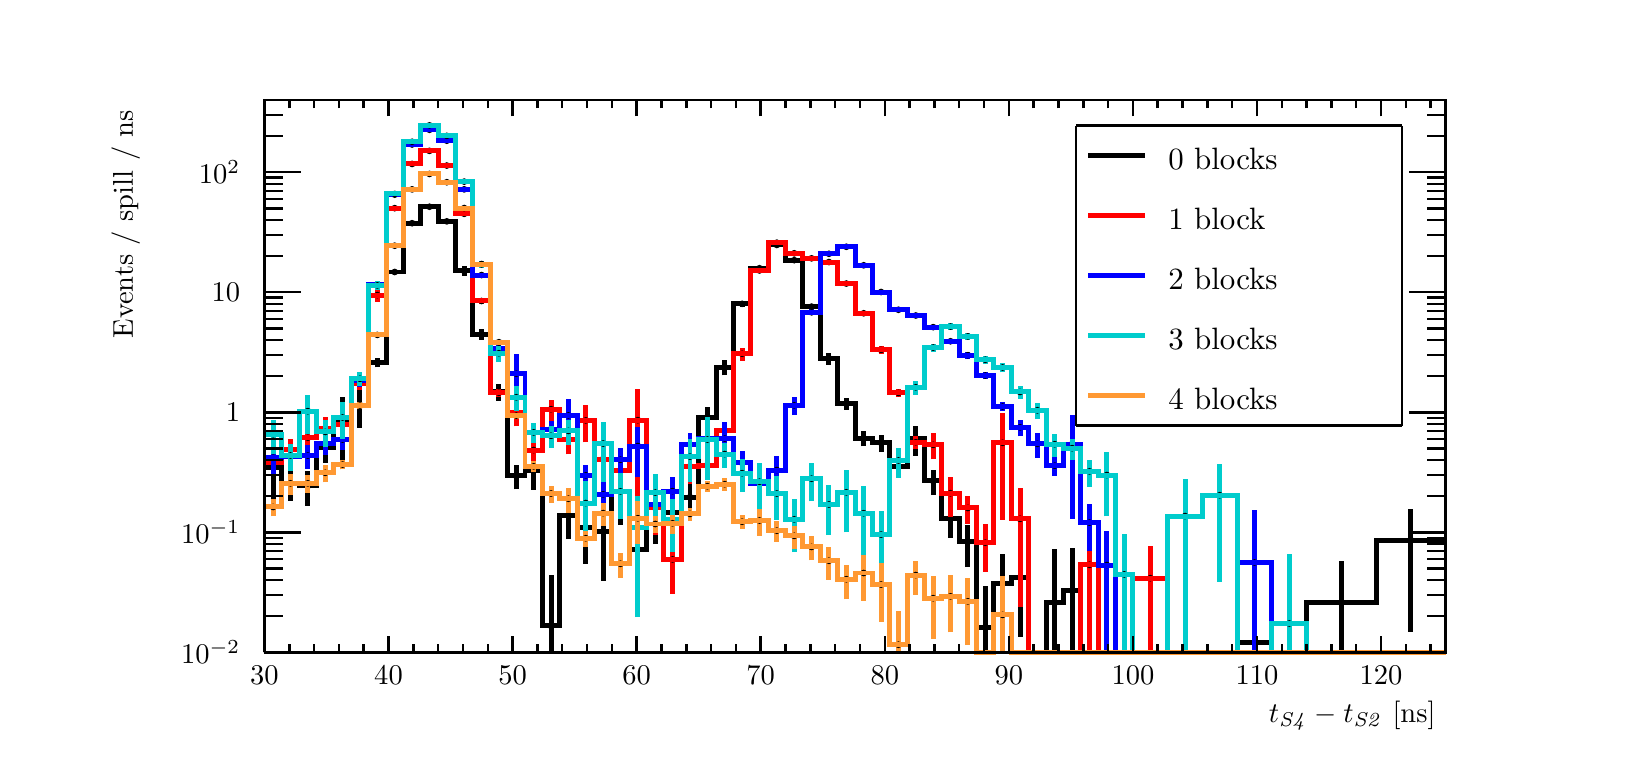
\begin{tikzpicture}
\pgfdeclareplotmark{cross} {
\pgfpathmoveto{\pgfpoint{-0.3\pgfplotmarksize}{\pgfplotmarksize}}
\pgfpathlineto{\pgfpoint{+0.3\pgfplotmarksize}{\pgfplotmarksize}}
\pgfpathlineto{\pgfpoint{+0.3\pgfplotmarksize}{0.3\pgfplotmarksize}}
\pgfpathlineto{\pgfpoint{+1\pgfplotmarksize}{0.3\pgfplotmarksize}}
\pgfpathlineto{\pgfpoint{+1\pgfplotmarksize}{-0.3\pgfplotmarksize}}
\pgfpathlineto{\pgfpoint{+0.3\pgfplotmarksize}{-0.3\pgfplotmarksize}}
\pgfpathlineto{\pgfpoint{+0.3\pgfplotmarksize}{-1.\pgfplotmarksize}}
\pgfpathlineto{\pgfpoint{-0.3\pgfplotmarksize}{-1.\pgfplotmarksize}}
\pgfpathlineto{\pgfpoint{-0.3\pgfplotmarksize}{-0.3\pgfplotmarksize}}
\pgfpathlineto{\pgfpoint{-1.\pgfplotmarksize}{-0.3\pgfplotmarksize}}
\pgfpathlineto{\pgfpoint{-1.\pgfplotmarksize}{0.3\pgfplotmarksize}}
\pgfpathlineto{\pgfpoint{-0.3\pgfplotmarksize}{0.3\pgfplotmarksize}}
\pgfpathclose
\pgfusepathqstroke
}
\pgfdeclareplotmark{cross*} {
\pgfpathmoveto{\pgfpoint{-0.3\pgfplotmarksize}{\pgfplotmarksize}}
\pgfpathlineto{\pgfpoint{+0.3\pgfplotmarksize}{\pgfplotmarksize}}
\pgfpathlineto{\pgfpoint{+0.3\pgfplotmarksize}{0.3\pgfplotmarksize}}
\pgfpathlineto{\pgfpoint{+1\pgfplotmarksize}{0.3\pgfplotmarksize}}
\pgfpathlineto{\pgfpoint{+1\pgfplotmarksize}{-0.3\pgfplotmarksize}}
\pgfpathlineto{\pgfpoint{+0.3\pgfplotmarksize}{-0.3\pgfplotmarksize}}
\pgfpathlineto{\pgfpoint{+0.3\pgfplotmarksize}{-1.\pgfplotmarksize}}
\pgfpathlineto{\pgfpoint{-0.3\pgfplotmarksize}{-1.\pgfplotmarksize}}
\pgfpathlineto{\pgfpoint{-0.3\pgfplotmarksize}{-0.3\pgfplotmarksize}}
\pgfpathlineto{\pgfpoint{-1.\pgfplotmarksize}{-0.3\pgfplotmarksize}}
\pgfpathlineto{\pgfpoint{-1.\pgfplotmarksize}{0.3\pgfplotmarksize}}
\pgfpathlineto{\pgfpoint{-0.3\pgfplotmarksize}{0.3\pgfplotmarksize}}
\pgfpathclose
\pgfusepathqfillstroke
}
\pgfdeclareplotmark{newstar} {
\pgfpathmoveto{\pgfqpoint{0pt}{\pgfplotmarksize}}
\pgfpathlineto{\pgfqpointpolar{44}{0.5\pgfplotmarksize}}
\pgfpathlineto{\pgfqpointpolar{18}{\pgfplotmarksize}}
\pgfpathlineto{\pgfqpointpolar{-20}{0.5\pgfplotmarksize}}
\pgfpathlineto{\pgfqpointpolar{-54}{\pgfplotmarksize}}
\pgfpathlineto{\pgfqpointpolar{-90}{0.5\pgfplotmarksize}}
\pgfpathlineto{\pgfqpointpolar{234}{\pgfplotmarksize}}
\pgfpathlineto{\pgfqpointpolar{198}{0.5\pgfplotmarksize}}
\pgfpathlineto{\pgfqpointpolar{162}{\pgfplotmarksize}}
\pgfpathlineto{\pgfqpointpolar{134}{0.5\pgfplotmarksize}}
\pgfpathclose
\pgfusepathqstroke
}
\pgfdeclareplotmark{newstar*} {
\pgfpathmoveto{\pgfqpoint{0pt}{\pgfplotmarksize}}
\pgfpathlineto{\pgfqpointpolar{44}{0.5\pgfplotmarksize}}
\pgfpathlineto{\pgfqpointpolar{18}{\pgfplotmarksize}}
\pgfpathlineto{\pgfqpointpolar{-20}{0.5\pgfplotmarksize}}
\pgfpathlineto{\pgfqpointpolar{-54}{\pgfplotmarksize}}
\pgfpathlineto{\pgfqpointpolar{-90}{0.5\pgfplotmarksize}}
\pgfpathlineto{\pgfqpointpolar{234}{\pgfplotmarksize}}
\pgfpathlineto{\pgfqpointpolar{198}{0.5\pgfplotmarksize}}
\pgfpathlineto{\pgfqpointpolar{162}{\pgfplotmarksize}}
\pgfpathlineto{\pgfqpointpolar{134}{0.5\pgfplotmarksize}}
\pgfpathclose
\pgfusepathqfillstroke
}
\definecolor{c}{rgb}{1,1,1};
\draw [color=c, fill=c] (0,0) rectangle (20,9.11025);
\draw [color=c, fill=c] (3,1.18433) rectangle (18,8.19923);
\definecolor{c}{rgb}{0,0,0};
\draw [c,line width=0.9] (3,1.18433) -- (3,8.19923) -- (18,8.19923) -- (18,1.18433) -- (3,1.18433);
\definecolor{c}{rgb}{1,1,1};
\draw [color=c, fill=c] (3,1.18433) rectangle (18,8.19923);
\definecolor{c}{rgb}{0,0,0};
\draw [c,line width=0.9] (3,1.18433) -- (3,8.19923) -- (18,8.19923) -- (18,1.18433) -- (3,1.18433);
\draw [c,line width=0.9] (3,1.18433) -- (3.22059,1.18433) -- (3.22059,1.18433) -- (3.44118,1.18433) -- (3.44118,1.18433) -- (3.66176,1.18433) -- (3.66176,1.18433) -- (3.88235,1.18433) -- (3.88235,1.18433) -- (4.10294,1.18433) -- (4.10294,1.18433) --
 (4.32353,1.18433) -- (4.32353,1.18433) -- (4.54412,1.18433) -- (4.54412,1.18433) -- (4.76471,1.18433) -- (4.76471,1.18433) -- (4.98529,1.18433) -- (4.98529,1.18433) -- (5.20588,1.18433) -- (5.20588,1.18433) -- (5.42647,1.18433) -- (5.42647,1.18433)
 -- (5.64706,1.18433) -- (5.64706,1.18433) -- (5.86765,1.18433) -- (5.86765,1.18433) -- (6.08824,1.18433) -- (6.08824,1.18433) -- (6.30882,1.18433) -- (6.30882,1.18433) -- (6.52941,1.18433) -- (6.52941,1.18433) -- (6.75,1.18433) -- (6.75,1.18433) --
 (6.97059,1.18433) -- (6.97059,1.18433) -- (7.19118,1.18433) -- (7.19118,1.18433) -- (7.41176,1.18433) -- (7.41176,1.18433) -- (7.63235,1.18433) -- (7.63235,1.18433) -- (7.85294,1.18433) -- (7.85294,1.18433) -- (8.07353,1.18433) -- (8.07353,1.18433)
 -- (8.29412,1.18433) -- (8.29412,1.18433) -- (8.51471,1.18433) -- (8.51471,1.18433) -- (8.73529,1.18433) -- (8.73529,1.18433) -- (8.95588,1.18433) -- (8.95588,1.18433) -- (9.17647,1.18433) -- (9.17647,1.18433) -- (9.39706,1.18433) --
 (9.39706,1.18433) -- (9.61765,1.18433) -- (9.61765,1.18433) -- (9.83823,1.18433) -- (9.83823,1.18433) -- (10.0588,1.18433) -- (10.0588,1.18433) -- (10.2794,1.18433) -- (10.2794,1.18433) -- (10.5,1.18433) -- (10.5,1.18433) -- (10.7206,1.18433) --
 (10.7206,1.18433) -- (10.9412,1.18433) -- (10.9412,1.18433) -- (11.1618,1.18433) -- (11.1618,1.18433) -- (11.3824,1.18433) -- (11.3824,1.18433) -- (11.6029,1.18433) -- (11.6029,1.18433) -- (11.8235,1.18433) -- (11.8235,1.18433) -- (12.0441,1.18433)
 -- (12.0441,1.18433) -- (12.2647,1.18433) -- (12.2647,1.18433) -- (12.4853,1.18433) -- (12.4853,1.18433) -- (12.7059,1.18433) -- (12.7059,1.18433) -- (12.9265,1.18433) -- (12.9265,1.18433) -- (13.1471,1.18433) -- (13.1471,1.18433) --
 (13.3676,1.18433) -- (13.3676,1.18433) -- (13.5882,1.18433) -- (13.5882,1.18433) -- (13.8088,1.18433) -- (13.8088,1.18433) -- (14.0294,1.18433) -- (14.0294,1.18433) -- (14.4706,1.18433) -- (14.4706,1.18433) -- (14.9118,1.18433) -- (14.9118,1.18433)
 -- (15.3529,1.18433) -- (15.3529,1.18433) -- (15.7941,1.18433) -- (15.7941,1.18433) -- (16.2353,1.18433) -- (16.2353,1.18433) -- (17.1176,1.18433) -- (17.1176,1.18433) -- (18,1.18433);
\draw [c,line width=0.9] (3,1.18433) -- (18,1.18433);
\draw [c,line width=0.9] (3,1.38931) -- (3,1.18433);
\draw [c,line width=0.9] (3.31513,1.28682) -- (3.31513,1.18433);
\draw [c,line width=0.9] (3.63025,1.28682) -- (3.63025,1.18433);
\draw [c,line width=0.9] (3.94538,1.28682) -- (3.94538,1.18433);
\draw [c,line width=0.9] (4.2605,1.28682) -- (4.2605,1.18433);
\draw [c,line width=0.9] (4.57563,1.38931) -- (4.57563,1.18433);
\draw [c,line width=0.9] (4.89076,1.28682) -- (4.89076,1.18433);
\draw [c,line width=0.9] (5.20588,1.28682) -- (5.20588,1.18433);
\draw [c,line width=0.9] (5.52101,1.28682) -- (5.52101,1.18433);
\draw [c,line width=0.9] (5.83613,1.28682) -- (5.83613,1.18433);
\draw [c,line width=0.9] (6.15126,1.38931) -- (6.15126,1.18433);
\draw [c,line width=0.9] (6.46639,1.28682) -- (6.46639,1.18433);
\draw [c,line width=0.9] (6.78151,1.28682) -- (6.78151,1.18433);
\draw [c,line width=0.9] (7.09664,1.28682) -- (7.09664,1.18433);
\draw [c,line width=0.9] (7.41176,1.28682) -- (7.41176,1.18433);
\draw [c,line width=0.9] (7.72689,1.38931) -- (7.72689,1.18433);
\draw [c,line width=0.9] (8.04202,1.28682) -- (8.04202,1.18433);
\draw [c,line width=0.9] (8.35714,1.28682) -- (8.35714,1.18433);
\draw [c,line width=0.9] (8.67227,1.28682) -- (8.67227,1.18433);
\draw [c,line width=0.9] (8.9874,1.28682) -- (8.9874,1.18433);
\draw [c,line width=0.9] (9.30252,1.38931) -- (9.30252,1.18433);
\draw [c,line width=0.9] (9.61765,1.28682) -- (9.61765,1.18433);
\draw [c,line width=0.9] (9.93277,1.28682) -- (9.93277,1.18433);
\draw [c,line width=0.9] (10.2479,1.28682) -- (10.2479,1.18433);
\draw [c,line width=0.9] (10.563,1.28682) -- (10.563,1.18433);
\draw [c,line width=0.9] (10.8782,1.38931) -- (10.8782,1.18433);
\draw [c,line width=0.9] (11.1933,1.28682) -- (11.1933,1.18433);
\draw [c,line width=0.9] (11.5084,1.28682) -- (11.5084,1.18433);
\draw [c,line width=0.9] (11.8235,1.28682) -- (11.8235,1.18433);
\draw [c,line width=0.9] (12.1387,1.28682) -- (12.1387,1.18433);
\draw [c,line width=0.9] (12.4538,1.38931) -- (12.4538,1.18433);
\draw [c,line width=0.9] (12.7689,1.28682) -- (12.7689,1.18433);
\draw [c,line width=0.9] (13.084,1.28682) -- (13.084,1.18433);
\draw [c,line width=0.9] (13.3992,1.28682) -- (13.3992,1.18433);
\draw [c,line width=0.9] (13.7143,1.28682) -- (13.7143,1.18433);
\draw [c,line width=0.9] (14.0294,1.38931) -- (14.0294,1.18433);
\draw [c,line width=0.9] (14.3445,1.28682) -- (14.3445,1.18433);
\draw [c,line width=0.9] (14.6597,1.28682) -- (14.6597,1.18433);
\draw [c,line width=0.9] (14.9748,1.28682) -- (14.9748,1.18433);
\draw [c,line width=0.9] (15.2899,1.28682) -- (15.2899,1.18433);
\draw [c,line width=0.9] (15.605,1.38931) -- (15.605,1.18433);
\draw [c,line width=0.9] (15.9202,1.28682) -- (15.9202,1.18433);
\draw [c,line width=0.9] (16.2353,1.28682) -- (16.2353,1.18433);
\draw [c,line width=0.9] (16.5504,1.28682) -- (16.5504,1.18433);
\draw [c,line width=0.9] (16.8655,1.28682) -- (16.8655,1.18433);
\draw [c,line width=0.9] (17.1807,1.38931) -- (17.1807,1.18433);
\draw [c,line width=0.9] (17.1807,1.38931) -- (17.1807,1.18433);
\draw [c,line width=0.9] (17.4958,1.28682) -- (17.4958,1.18433);
\draw [c,line width=0.9] (17.8109,1.28682) -- (17.8109,1.18433);
\draw [anchor=base] (3,0.774371) node[scale=1.03101, color=c, rotate=0]{30};
\draw [anchor=base] (4.57563,0.774371) node[scale=1.03101, color=c, rotate=0]{40};
\draw [anchor=base] (6.15126,0.774371) node[scale=1.03101, color=c, rotate=0]{50};
\draw [anchor=base] (7.72689,0.774371) node[scale=1.03101, color=c, rotate=0]{60};
\draw [anchor=base] (9.30252,0.774371) node[scale=1.03101, color=c, rotate=0]{70};
\draw [anchor=base] (10.8782,0.774371) node[scale=1.03101, color=c, rotate=0]{80};
\draw [anchor=base] (12.4538,0.774371) node[scale=1.03101, color=c, rotate=0]{90};
\draw [anchor=base] (14.0294,0.774371) node[scale=1.03101, color=c, rotate=0]{100};
\draw [anchor=base] (15.605,0.774371) node[scale=1.03101, color=c, rotate=0]{110};
\draw [anchor=base] (17.1807,0.774371) node[scale=1.03101, color=c, rotate=0]{120};
\draw [anchor= east] (18,0.382631) node[scale=1.03101, color=c, rotate=0]{$ t_{\mathit{S4}} - t_{\mathit{S2}}$ [ns]};
\draw [c,line width=0.9] (3,8.19923) -- (18,8.19923);
\draw [c,line width=0.9] (3,7.99425) -- (3,8.19923);
\draw [c,line width=0.9] (3.31513,8.09674) -- (3.31513,8.19923);
\draw [c,line width=0.9] (3.63025,8.09674) -- (3.63025,8.19923);
\draw [c,line width=0.9] (3.94538,8.09674) -- (3.94538,8.19923);
\draw [c,line width=0.9] (4.2605,8.09674) -- (4.2605,8.19923);
\draw [c,line width=0.9] (4.57563,7.99425) -- (4.57563,8.19923);
\draw [c,line width=0.9] (4.89076,8.09674) -- (4.89076,8.19923);
\draw [c,line width=0.9] (5.20588,8.09674) -- (5.20588,8.19923);
\draw [c,line width=0.9] (5.52101,8.09674) -- (5.52101,8.19923);
\draw [c,line width=0.9] (5.83613,8.09674) -- (5.83613,8.19923);
\draw [c,line width=0.9] (6.15126,7.99425) -- (6.15126,8.19923);
\draw [c,line width=0.9] (6.46639,8.09674) -- (6.46639,8.19923);
\draw [c,line width=0.9] (6.78151,8.09674) -- (6.78151,8.19923);
\draw [c,line width=0.9] (7.09664,8.09674) -- (7.09664,8.19923);
\draw [c,line width=0.9] (7.41176,8.09674) -- (7.41176,8.19923);
\draw [c,line width=0.9] (7.72689,7.99425) -- (7.72689,8.19923);
\draw [c,line width=0.9] (8.04202,8.09674) -- (8.04202,8.19923);
\draw [c,line width=0.9] (8.35714,8.09674) -- (8.35714,8.19923);
\draw [c,line width=0.9] (8.67227,8.09674) -- (8.67227,8.19923);
\draw [c,line width=0.9] (8.9874,8.09674) -- (8.9874,8.19923);
\draw [c,line width=0.9] (9.30252,7.99425) -- (9.30252,8.19923);
\draw [c,line width=0.9] (9.61765,8.09674) -- (9.61765,8.19923);
\draw [c,line width=0.9] (9.93277,8.09674) -- (9.93277,8.19923);
\draw [c,line width=0.9] (10.2479,8.09674) -- (10.2479,8.19923);
\draw [c,line width=0.9] (10.563,8.09674) -- (10.563,8.19923);
\draw [c,line width=0.9] (10.8782,7.99425) -- (10.8782,8.19923);
\draw [c,line width=0.9] (11.1933,8.09674) -- (11.1933,8.19923);
\draw [c,line width=0.9] (11.5084,8.09674) -- (11.5084,8.19923);
\draw [c,line width=0.9] (11.8235,8.09674) -- (11.8235,8.19923);
\draw [c,line width=0.9] (12.1387,8.09674) -- (12.1387,8.19923);
\draw [c,line width=0.9] (12.4538,7.99425) -- (12.4538,8.19923);
\draw [c,line width=0.9] (12.7689,8.09674) -- (12.7689,8.19923);
\draw [c,line width=0.9] (13.084,8.09674) -- (13.084,8.19923);
\draw [c,line width=0.9] (13.3992,8.09674) -- (13.3992,8.19923);
\draw [c,line width=0.9] (13.7143,8.09674) -- (13.7143,8.19923);
\draw [c,line width=0.9] (14.0294,7.99425) -- (14.0294,8.19923);
\draw [c,line width=0.9] (14.3445,8.09674) -- (14.3445,8.19923);
\draw [c,line width=0.9] (14.6597,8.09674) -- (14.6597,8.19923);
\draw [c,line width=0.9] (14.9748,8.09674) -- (14.9748,8.19923);
\draw [c,line width=0.9] (15.2899,8.09674) -- (15.2899,8.19923);
\draw [c,line width=0.9] (15.605,7.99425) -- (15.605,8.19923);
\draw [c,line width=0.9] (15.9202,8.09674) -- (15.9202,8.19923);
\draw [c,line width=0.9] (16.2353,8.09674) -- (16.2353,8.19923);
\draw [c,line width=0.9] (16.5504,8.09674) -- (16.5504,8.19923);
\draw [c,line width=0.9] (16.8655,8.09674) -- (16.8655,8.19923);
\draw [c,line width=0.9] (17.1807,7.99425) -- (17.1807,8.19923);
\draw [c,line width=0.9] (17.1807,7.99425) -- (17.1807,8.19923);
\draw [c,line width=0.9] (17.4958,8.09674) -- (17.4958,8.19923);
\draw [c,line width=0.9] (17.8109,8.09674) -- (17.8109,8.19923);
\draw [c,line width=0.9] (3,1.18433) -- (3,8.19923);
\draw [c,line width=0.9] (3.462,1.18433) -- (3,1.18433);
\draw [anchor= east] (2.82,1.18433) node[scale=1.03101, color=c, rotate=0]{$10^{-2}$};
\draw [c,line width=0.9] (3.231,1.64319) -- (3,1.64319);
\draw [c,line width=0.9] (3.231,1.91161) -- (3,1.91161);
\draw [c,line width=0.9] (3.231,2.10205) -- (3,2.10205);
\draw [c,line width=0.9] (3.231,2.24977) -- (3,2.24977);
\draw [c,line width=0.9] (3.231,2.37047) -- (3,2.37047);
\draw [c,line width=0.9] (3.231,2.47251) -- (3,2.47251);
\draw [c,line width=0.9] (3.231,2.56091) -- (3,2.56091);
\draw [c,line width=0.9] (3.231,2.63888) -- (3,2.63888);
\draw [c,line width=0.9] (3.462,2.70863) -- (3,2.70863);
\draw [anchor= east] (2.82,2.70863) node[scale=1.03101, color=c, rotate=0]{$10^{-1}$};
\draw [c,line width=0.9] (3.231,3.16749) -- (3,3.16749);
\draw [c,line width=0.9] (3.231,3.4359) -- (3,3.4359);
\draw [c,line width=0.9] (3.231,3.62634) -- (3,3.62634);
\draw [c,line width=0.9] (3.231,3.77406) -- (3,3.77406);
\draw [c,line width=0.9] (3.231,3.89476) -- (3,3.89476);
\draw [c,line width=0.9] (3.231,3.99681) -- (3,3.99681);
\draw [c,line width=0.9] (3.231,4.0852) -- (3,4.0852);
\draw [c,line width=0.9] (3.231,4.16317) -- (3,4.16317);
\draw [c,line width=0.9] (3.462,4.23292) -- (3,4.23292);
\draw [anchor= east] (2.82,4.23292) node[scale=1.03101, color=c, rotate=0]{1};
\draw [c,line width=0.9] (3.231,4.69178) -- (3,4.69178);
\draw [c,line width=0.9] (3.231,4.9602) -- (3,4.9602);
\draw [c,line width=0.9] (3.231,5.15064) -- (3,5.15064);
\draw [c,line width=0.9] (3.231,5.29836) -- (3,5.29836);
\draw [c,line width=0.9] (3.231,5.41905) -- (3,5.41905);
\draw [c,line width=0.9] (3.231,5.5211) -- (3,5.5211);
\draw [c,line width=0.9] (3.231,5.6095) -- (3,5.6095);
\draw [c,line width=0.9] (3.231,5.68747) -- (3,5.68747);
\draw [c,line width=0.9] (3.462,5.75722) -- (3,5.75722);
\draw [anchor= east] (2.82,5.75722) node[scale=1.03101, color=c, rotate=0]{10};
\draw [c,line width=0.9] (3.231,6.21607) -- (3,6.21607);
\draw [c,line width=0.9] (3.231,6.48449) -- (3,6.48449);
\draw [c,line width=0.9] (3.231,6.67493) -- (3,6.67493);
\draw [c,line width=0.9] (3.231,6.82265) -- (3,6.82265);
\draw [c,line width=0.9] (3.231,6.94335) -- (3,6.94335);
\draw [c,line width=0.9] (3.231,7.04539) -- (3,7.04539);
\draw [c,line width=0.9] (3.231,7.13379) -- (3,7.13379);
\draw [c,line width=0.9] (3.231,7.21176) -- (3,7.21176);
\draw [c,line width=0.9] (3.462,7.28151) -- (3,7.28151);
\draw [anchor= east] (2.82,7.28151) node[scale=1.03101, color=c, rotate=0]{$10^{2}$};
\draw [c,line width=0.9] (3.231,7.74037) -- (3,7.74037);
\draw [c,line width=0.9] (3.231,8.00878) -- (3,8.00878);
\draw [c,line width=0.9] (3.231,8.19923) -- (3,8.19923);
\draw [anchor= east] (1.24,8.19923) node[scale=1.03101, color=c, rotate=90]{ Events / spill / ns};
\draw [c,line width=0.9] (18,1.18433) -- (18,8.19923);
\draw [c,line width=0.9] (17.538,1.18433) -- (18,1.18433);
\draw [c,line width=0.9] (17.769,1.64319) -- (18,1.64319);
\draw [c,line width=0.9] (17.769,1.91161) -- (18,1.91161);
\draw [c,line width=0.9] (17.769,2.10205) -- (18,2.10205);
\draw [c,line width=0.9] (17.769,2.24977) -- (18,2.24977);
\draw [c,line width=0.9] (17.769,2.37047) -- (18,2.37047);
\draw [c,line width=0.9] (17.769,2.47251) -- (18,2.47251);
\draw [c,line width=0.9] (17.769,2.56091) -- (18,2.56091);
\draw [c,line width=0.9] (17.769,2.63888) -- (18,2.63888);
\draw [c,line width=0.9] (17.538,2.70863) -- (18,2.70863);
\draw [c,line width=0.9] (17.769,3.16749) -- (18,3.16749);
\draw [c,line width=0.9] (17.769,3.4359) -- (18,3.4359);
\draw [c,line width=0.9] (17.769,3.62634) -- (18,3.62634);
\draw [c,line width=0.9] (17.769,3.77406) -- (18,3.77406);
\draw [c,line width=0.9] (17.769,3.89476) -- (18,3.89476);
\draw [c,line width=0.9] (17.769,3.99681) -- (18,3.99681);
\draw [c,line width=0.9] (17.769,4.0852) -- (18,4.0852);
\draw [c,line width=0.9] (17.769,4.16317) -- (18,4.16317);
\draw [c,line width=0.9] (17.538,4.23292) -- (18,4.23292);
\draw [c,line width=0.9] (17.769,4.69178) -- (18,4.69178);
\draw [c,line width=0.9] (17.769,4.9602) -- (18,4.9602);
\draw [c,line width=0.9] (17.769,5.15064) -- (18,5.15064);
\draw [c,line width=0.9] (17.769,5.29836) -- (18,5.29836);
\draw [c,line width=0.9] (17.769,5.41905) -- (18,5.41905);
\draw [c,line width=0.9] (17.769,5.5211) -- (18,5.5211);
\draw [c,line width=0.9] (17.769,5.6095) -- (18,5.6095);
\draw [c,line width=0.9] (17.769,5.68747) -- (18,5.68747);
\draw [c,line width=0.9] (17.538,5.75722) -- (18,5.75722);
\draw [c,line width=0.9] (17.769,6.21607) -- (18,6.21607);
\draw [c,line width=0.9] (17.769,6.48449) -- (18,6.48449);
\draw [c,line width=0.9] (17.769,6.67493) -- (18,6.67493);
\draw [c,line width=0.9] (17.769,6.82265) -- (18,6.82265);
\draw [c,line width=0.9] (17.769,6.94335) -- (18,6.94335);
\draw [c,line width=0.9] (17.769,7.04539) -- (18,7.04539);
\draw [c,line width=0.9] (17.769,7.13379) -- (18,7.13379);
\draw [c,line width=0.9] (17.769,7.21176) -- (18,7.21176);
\draw [c,line width=0.9] (17.538,7.28151) -- (18,7.28151);
\draw [c,line width=0.9] (17.769,7.74037) -- (18,7.74037);
\draw [c,line width=0.9] (17.769,8.00878) -- (18,8.00878);
\draw [c,line width=0.9] (17.769,8.19923) -- (18,8.19923);
\draw [c,line width=1.8] (3.11029,3.01059) -- (3.11029,3.53716);
\draw [c,line width=1.8] (3.11029,3.53716) -- (3.11029,3.82669);
\foreach \P in {(3.11029,3.53716)}{\draw[mark options={color=c,fill=c},mark size=2.402402pt,mark=*,mark size=1pt] plot coordinates {\P};}
\draw [c,line width=1.8] (3.33088,3.11042) -- (3.33088,3.3234);
\draw [c,line width=1.8] (3.33088,3.3234) -- (3.33088,3.48428);
\foreach \P in {(3.33088,3.3234)}{\draw[mark options={color=c,fill=c},mark size=2.402402pt,mark=*,mark size=1pt] plot coordinates {\P};}
\draw [c,line width=1.8] (3.55147,3.04626) -- (3.55147,3.29901);
\draw [c,line width=1.8] (3.55147,3.29901) -- (3.55147,3.48149);
\foreach \P in {(3.55147,3.29901)}{\draw[mark options={color=c,fill=c},mark size=2.402402pt,mark=*,mark size=1pt] plot coordinates {\P};}
\draw [c,line width=1.8] (3.77206,3.59376) -- (3.77206,3.78886);
\draw [c,line width=1.8] (3.77206,3.78886) -- (3.77206,3.93936);
\foreach \P in {(3.77206,3.78886)}{\draw[mark options={color=c,fill=c},mark size=2.402402pt,mark=*,mark size=1pt] plot coordinates {\P};}
\draw [c,line width=1.8] (3.99265,3.50647) -- (3.99265,4.11906);
\draw [c,line width=1.8] (3.99265,4.11906) -- (3.99265,4.4317);
\foreach \P in {(3.99265,4.11906)}{\draw[mark options={color=c,fill=c},mark size=2.402402pt,mark=*,mark size=1pt] plot coordinates {\P};}
\draw [c,line width=1.8] (4.21324,4.03848) -- (4.21324,4.32444);
\draw [c,line width=1.8] (4.21324,4.32444) -- (4.21324,4.52349);
\foreach \P in {(4.21324,4.32444)}{\draw[mark options={color=c,fill=c},mark size=2.402402pt,mark=*,mark size=1pt] plot coordinates {\P};}
\draw [c,line width=1.8] (4.43382,4.80441) -- (4.43382,4.86726);
\draw [c,line width=1.8] (4.43382,4.86726) -- (4.43382,4.92466);
\foreach \P in {(4.43382,4.86726)}{\draw[mark options={color=c,fill=c},mark size=2.402402pt,mark=*,mark size=1pt] plot coordinates {\P};}
\draw [c,line width=1.8] (4.65441,5.98509) -- (4.65441,6.01435);
\draw [c,line width=1.8] (4.65441,6.01435) -- (4.65441,6.04237);
\foreach \P in {(4.65441,6.01435)}{\draw[mark options={color=c,fill=c},mark size=2.402402pt,mark=*,mark size=1pt] plot coordinates {\P};}
\draw [c,line width=1.8] (4.875,6.6125) -- (4.875,6.63394);
\draw [c,line width=1.8] (4.875,6.63394) -- (4.875,6.65471);
\foreach \P in {(4.875,6.63394)}{\draw[mark options={color=c,fill=c},mark size=2.402402pt,mark=*,mark size=1pt] plot coordinates {\P};}
\draw [c,line width=1.8] (5.09559,6.82128) -- (5.09559,6.84324);
\draw [c,line width=1.8] (5.09559,6.84324) -- (5.09559,6.8645);
\foreach \P in {(5.09559,6.84324)}{\draw[mark options={color=c,fill=c},mark size=2.402402pt,mark=*,mark size=1pt] plot coordinates {\P};}
\draw [c,line width=1.8] (5.31618,6.62665) -- (5.31618,6.65758);
\draw [c,line width=1.8] (5.31618,6.65758) -- (5.31618,6.68713);
\foreach \P in {(5.31618,6.65758)}{\draw[mark options={color=c,fill=c},mark size=2.402402pt,mark=*,mark size=1pt] plot coordinates {\P};}
\draw [c,line width=1.8] (5.53676,5.96974) -- (5.53676,6.02947);
\draw [c,line width=1.8] (5.53676,6.02947) -- (5.53676,6.08426);
\foreach \P in {(5.53676,6.02947)}{\draw[mark options={color=c,fill=c},mark size=2.402402pt,mark=*,mark size=1pt] plot coordinates {\P};}
\draw [c,line width=1.8] (5.75735,5.15161) -- (5.75735,5.22451);
\draw [c,line width=1.8] (5.75735,5.22451) -- (5.75735,5.29016);
\foreach \P in {(5.75735,5.22451)}{\draw[mark options={color=c,fill=c},mark size=2.402402pt,mark=*,mark size=1pt] plot coordinates {\P};}
\draw [c,line width=1.8] (5.97794,4.37808) -- (5.97794,4.49492);
\draw [c,line width=1.8] (5.97794,4.49492) -- (5.97794,4.5942);
\foreach \P in {(5.97794,4.49492)}{\draw[mark options={color=c,fill=c},mark size=2.402402pt,mark=*,mark size=1pt] plot coordinates {\P};}
\draw [c,line width=1.8] (6.19853,3.25269) -- (6.19853,3.42437);
\draw [c,line width=1.8] (6.19853,3.42437) -- (6.19853,3.56058);
\foreach \P in {(6.19853,3.42437)}{\draw[mark options={color=c,fill=c},mark size=2.402402pt,mark=*,mark size=1pt] plot coordinates {\P};}
\draw [c,line width=1.8] (6.41912,3.25055) -- (6.41912,3.49418);
\draw [c,line width=1.8] (6.41912,3.49418) -- (6.41912,3.67187);
\foreach \P in {(6.41912,3.49418)}{\draw[mark options={color=c,fill=c},mark size=2.402402pt,mark=*,mark size=1pt] plot coordinates {\P};}
\draw [c,line width=1.8] (6.63971,1.18433) -- (6.63971,1.52013);
\draw [c,line width=1.8] (6.63971,1.52013) -- (6.63971,2.16651);
\foreach \P in {(6.63971,1.52013)}{\draw[mark options={color=c,fill=c},mark size=2.402402pt,mark=*,mark size=1pt] plot coordinates {\P};}
\draw [c,line width=1.8] (6.86029,2.6208) -- (6.86029,2.92257);
\draw [c,line width=1.8] (6.86029,2.92257) -- (6.86029,3.12908);
\foreach \P in {(6.86029,2.92257)}{\draw[mark options={color=c,fill=c},mark size=2.402402pt,mark=*,mark size=1pt] plot coordinates {\P};}
\draw [c,line width=1.8] (7.08088,2.30724) -- (7.08088,2.76685);
\draw [c,line width=1.8] (7.08088,2.76685) -- (7.08088,3.03552);
\foreach \P in {(7.08088,2.76685)}{\draw[mark options={color=c,fill=c},mark size=2.402402pt,mark=*,mark size=1pt] plot coordinates {\P};}
\draw [c,line width=1.8] (7.30147,2.09583) -- (7.30147,2.71841);
\draw [c,line width=1.8] (7.30147,2.71841) -- (7.30147,3.03349);
\foreach \P in {(7.30147,2.71841)}{\draw[mark options={color=c,fill=c},mark size=2.402402pt,mark=*,mark size=1pt] plot coordinates {\P};}
\draw [c,line width=1.8] (7.52206,2.80159) -- (7.52206,3.22686);
\draw [c,line width=1.8] (7.52206,3.22686) -- (7.52206,3.48368);
\foreach \P in {(7.52206,3.22686)}{\draw[mark options={color=c,fill=c},mark size=2.402402pt,mark=*,mark size=1pt] plot coordinates {\P};}
\draw [c,line width=1.8] (7.74265,2.00764) -- (7.74265,2.49321);
\draw [c,line width=1.8] (7.74265,2.49321) -- (7.74265,2.7703);
\foreach \P in {(7.74265,2.49321)}{\draw[mark options={color=c,fill=c},mark size=2.402402pt,mark=*,mark size=1pt] plot coordinates {\P};}
\draw [c,line width=1.8] (7.96324,2.55851) -- (7.96324,3.02649);
\draw [c,line width=1.8] (7.96324,3.02649) -- (7.96324,3.29792);
\foreach \P in {(7.96324,3.02649)}{\draw[mark options={color=c,fill=c},mark size=2.402402pt,mark=*,mark size=1pt] plot coordinates {\P};}
\draw [c,line width=1.8] (8.18382,2.65833) -- (8.18382,2.95996);
\draw [c,line width=1.8] (8.18382,2.95996) -- (8.18382,3.16641);
\foreach \P in {(8.18382,2.95996)}{\draw[mark options={color=c,fill=c},mark size=2.402402pt,mark=*,mark size=1pt] plot coordinates {\P};}
\draw [c,line width=1.8] (8.40441,2.93473) -- (8.40441,3.15503);
\draw [c,line width=1.8] (8.40441,3.15503) -- (8.40441,3.32004);
\foreach \P in {(8.40441,3.15503)}{\draw[mark options={color=c,fill=c},mark size=2.402402pt,mark=*,mark size=1pt] plot coordinates {\P};}
\draw [c,line width=1.8] (8.625,4.01263) -- (8.625,4.17078);
\draw [c,line width=1.8] (8.625,4.17078) -- (8.625,4.29834);
\foreach \P in {(8.625,4.17078)}{\draw[mark options={color=c,fill=c},mark size=2.402402pt,mark=*,mark size=1pt] plot coordinates {\P};}
\draw [c,line width=1.8] (8.84559,4.70224) -- (8.84559,4.8068);
\draw [c,line width=1.8] (8.84559,4.8068) -- (8.84559,4.89707);
\foreach \P in {(8.84559,4.8068)}{\draw[mark options={color=c,fill=c},mark size=2.402402pt,mark=*,mark size=1pt] plot coordinates {\P};}
\draw [c,line width=1.8] (9.06618,5.56733) -- (9.06618,5.6099);
\draw [c,line width=1.8] (9.06618,5.6099) -- (9.06618,5.64989);
\foreach \P in {(9.06618,5.6099)}{\draw[mark options={color=c,fill=c},mark size=2.402402pt,mark=*,mark size=1pt] plot coordinates {\P};}
\draw [c,line width=1.8] (9.28677,6.03393) -- (9.28677,6.06192);
\draw [c,line width=1.8] (9.28677,6.06192) -- (9.28677,6.08878);
\foreach \P in {(9.28677,6.06192)}{\draw[mark options={color=c,fill=c},mark size=2.402402pt,mark=*,mark size=1pt] plot coordinates {\P};}
\draw [c,line width=1.8] (9.50735,6.33726) -- (9.50735,6.35795);
\draw [c,line width=1.8] (9.50735,6.35795) -- (9.50735,6.37801);
\foreach \P in {(9.50735,6.35795)}{\draw[mark options={color=c,fill=c},mark size=2.402402pt,mark=*,mark size=1pt] plot coordinates {\P};}
\draw [c,line width=1.8] (9.72794,6.14261) -- (9.72794,6.16458);
\draw [c,line width=1.8] (9.72794,6.16458) -- (9.72794,6.18584);
\foreach \P in {(9.72794,6.16458)}{\draw[mark options={color=c,fill=c},mark size=2.402402pt,mark=*,mark size=1pt] plot coordinates {\P};}
\draw [c,line width=1.8] (9.94853,5.53971) -- (9.94853,5.57486);
\draw [c,line width=1.8] (9.94853,5.57486) -- (9.94853,5.60823);
\foreach \P in {(9.94853,5.57486)}{\draw[mark options={color=c,fill=c},mark size=2.402402pt,mark=*,mark size=1pt] plot coordinates {\P};}
\draw [c,line width=1.8] (10.1691,4.83738) -- (10.1691,4.9182);
\draw [c,line width=1.8] (10.1691,4.9182) -- (10.1691,4.99022);
\foreach \P in {(10.1691,4.9182)}{\draw[mark options={color=c,fill=c},mark size=2.402402pt,mark=*,mark size=1pt] plot coordinates {\P};}
\draw [c,line width=1.8] (10.3897,4.26375) -- (10.3897,4.33999);
\draw [c,line width=1.8] (10.3897,4.33999) -- (10.3897,4.40834);
\foreach \P in {(10.3897,4.33999)}{\draw[mark options={color=c,fill=c},mark size=2.402402pt,mark=*,mark size=1pt] plot coordinates {\P};}
\draw [c,line width=1.8] (10.6103,3.79985) -- (10.6103,3.9013);
\draw [c,line width=1.8] (10.6103,3.9013) -- (10.6103,3.98925);
\foreach \P in {(10.6103,3.9013)}{\draw[mark options={color=c,fill=c},mark size=2.402402pt,mark=*,mark size=1pt] plot coordinates {\P};}
\draw [c,line width=1.8] (10.8309,3.72814) -- (10.8309,3.84562);
\draw [c,line width=1.8] (10.8309,3.84562) -- (10.8309,3.94536);
\foreach \P in {(10.8309,3.84562)}{\draw[mark options={color=c,fill=c},mark size=2.402402pt,mark=*,mark size=1pt] plot coordinates {\P};}
\draw [c,line width=1.8] (11.0515,3.40787) -- (11.0515,3.53943);
\draw [c,line width=1.8] (11.0515,3.53943) -- (11.0515,3.64913);
\foreach \P in {(11.0515,3.53943)}{\draw[mark options={color=c,fill=c},mark size=2.402402pt,mark=*,mark size=1pt] plot coordinates {\P};}
\draw [c,line width=1.8] (11.2721,3.6794) -- (11.2721,3.89767);
\draw [c,line width=1.8] (11.2721,3.89767) -- (11.2721,4.06153);
\foreach \P in {(11.2721,3.89767)}{\draw[mark options={color=c,fill=c},mark size=2.402402pt,mark=*,mark size=1pt] plot coordinates {\P};}
\draw [c,line width=1.8] (11.4926,3.17961) -- (11.4926,3.36034);
\draw [c,line width=1.8] (11.4926,3.36034) -- (11.4926,3.50216);
\foreach \P in {(11.4926,3.36034)}{\draw[mark options={color=c,fill=c},mark size=2.402402pt,mark=*,mark size=1pt] plot coordinates {\P};}
\draw [c,line width=1.8] (11.7132,2.64028) -- (11.7132,2.88433);
\draw [c,line width=1.8] (11.7132,2.88433) -- (11.7132,3.06225);
\foreach \P in {(11.7132,2.88433)}{\draw[mark options={color=c,fill=c},mark size=2.402402pt,mark=*,mark size=1pt] plot coordinates {\P};}
\draw [c,line width=1.8] (11.9338,2.26532) -- (11.9338,2.59007);
\draw [c,line width=1.8] (11.9338,2.59007) -- (11.9338,2.80697);
\foreach \P in {(11.9338,2.59007)}{\draw[mark options={color=c,fill=c},mark size=2.402402pt,mark=*,mark size=1pt] plot coordinates {\P};}
\draw [c,line width=1.8] (12.1544,1.18433) -- (12.1544,1.50181);
\draw [c,line width=1.8] (12.1544,1.50181) -- (12.1544,2.02432);
\foreach \P in {(12.1544,1.50181)}{\draw[mark options={color=c,fill=c},mark size=2.402402pt,mark=*,mark size=1pt] plot coordinates {\P};}
\draw [c,line width=1.8] (12.375,1.18433) -- (12.375,2.05707);
\draw [c,line width=1.8] (12.375,2.05707) -- (12.375,2.42814);
\foreach \P in {(12.375,2.05707)}{\draw[mark options={color=c,fill=c},mark size=2.402402pt,mark=*,mark size=1pt] plot coordinates {\P};}
\draw [c,line width=1.8] (12.5956,1.38032) -- (12.5956,2.13491);
\draw [c,line width=1.8] (12.5956,2.13491) -- (12.5956,2.4784);
\foreach \P in {(12.5956,2.13491)}{\draw[mark options={color=c,fill=c},mark size=2.402402pt,mark=*,mark size=1pt] plot coordinates {\P};}
\draw [c,line width=1.8] (13.0368,1.18433) -- (13.0368,1.81278);
\draw [c,line width=1.8] (13.0368,1.81278) -- (13.0368,2.49098);
\foreach \P in {(13.0368,1.81278)}{\draw[mark options={color=c,fill=c},mark size=2.402402pt,mark=*,mark size=1pt] plot coordinates {\P};}
\draw [c,line width=1.8] (13.2574,1.18433) -- (13.2574,1.96775);
\draw [c,line width=1.8] (13.2574,1.96775) -- (13.2574,2.508);
\foreach \P in {(13.2574,1.96775)}{\draw[mark options={color=c,fill=c},mark size=2.402402pt,mark=*,mark size=1pt] plot coordinates {\P};}
\draw [c,line width=1.8] (15.5735,1.18433) -- (15.5735,1.30488);
\draw [c,line width=1.8] (15.5735,1.30488) -- (15.5735,2.1569);
\foreach \P in {(15.5735,1.30488)}{\draw[mark options={color=c,fill=c},mark size=2.402402pt,mark=*,mark size=1pt] plot coordinates {\P};}
\draw [c,line width=1.8] (16.6765,1.18433) -- (16.6765,1.81474);
\draw [c,line width=1.8] (16.6765,1.81474) -- (16.6765,2.34592);
\foreach \P in {(16.6765,1.81474)}{\draw[mark options={color=c,fill=c},mark size=2.402402pt,mark=*,mark size=1pt] plot coordinates {\P};}
\draw [c,line width=1.8] (17.5588,1.44788) -- (17.5588,2.60963);
\draw [c,line width=1.8] (17.5588,2.60963) -- (17.5588,3.00863);
\foreach \P in {(17.5588,2.60963)}{\draw[mark options={color=c,fill=c},mark size=2.402402pt,mark=*,mark size=1pt] plot coordinates {\P};}
\draw [c,line width=1.8] (3,3.53716) -- (3.22059,3.53716) -- (3.22059,3.3234) -- (3.44118,3.3234) -- (3.44118,3.29901) -- (3.66176,3.29901) -- (3.66176,3.78886) -- (3.88235,3.78886) -- (3.88235,4.11906) -- (4.10294,4.11906) -- (4.10294,4.32444) --
 (4.32353,4.32444) -- (4.32353,4.86726) -- (4.54412,4.86726) -- (4.54412,6.01435) -- (4.76471,6.01435) -- (4.76471,6.63394) -- (4.98529,6.63394) -- (4.98529,6.84324) -- (5.20588,6.84324) -- (5.20588,6.65758) -- (5.42647,6.65758) -- (5.42647,6.02947)
 -- (5.64706,6.02947) -- (5.64706,5.22451) -- (5.86765,5.22451) -- (5.86765,4.49492) -- (6.08824,4.49492) -- (6.08824,3.42437) -- (6.30882,3.42437) -- (6.30882,3.49418) -- (6.52941,3.49418) -- (6.52941,1.52013) -- (6.75,1.52013) -- (6.75,2.92257) --
 (6.97059,2.92257) -- (6.97059,2.76685) -- (7.19118,2.76685) -- (7.19118,2.71841) -- (7.41176,2.71841) -- (7.41176,3.22686) -- (7.63235,3.22686) -- (7.63235,2.49321) -- (7.85294,2.49321) -- (7.85294,3.02649) -- (8.07353,3.02649) -- (8.07353,2.95996)
 -- (8.29412,2.95996) -- (8.29412,3.15503) -- (8.51471,3.15503) -- (8.51471,4.17078) -- (8.73529,4.17078) -- (8.73529,4.8068) -- (8.95588,4.8068) -- (8.95588,5.6099) -- (9.17647,5.6099) -- (9.17647,6.06192) -- (9.39706,6.06192) -- (9.39706,6.35795)
 -- (9.61765,6.35795) -- (9.61765,6.16458) -- (9.83823,6.16458) -- (9.83823,5.57486) -- (10.0588,5.57486) -- (10.0588,4.9182) -- (10.2794,4.9182) -- (10.2794,4.33999) -- (10.5,4.33999) -- (10.5,3.9013) -- (10.7206,3.9013) -- (10.7206,3.84562) --
 (10.9412,3.84562) -- (10.9412,3.53943) -- (11.1618,3.53943) -- (11.1618,3.89767) -- (11.3824,3.89767) -- (11.3824,3.36034) -- (11.6029,3.36034) -- (11.6029,2.88433) -- (11.8235,2.88433) -- (11.8235,2.59007) -- (12.0441,2.59007) -- (12.0441,1.50181)
 -- (12.2647,1.50181) -- (12.2647,2.05707) -- (12.4853,2.05707) -- (12.4853,2.13491) -- (12.7059,2.13491) -- (12.7059,1.18433) -- (12.9265,1.18433) -- (12.9265,1.81278) -- (13.1471,1.81278) -- (13.1471,1.96775) -- (13.3676,1.96775) --
 (13.3676,1.18433) -- (13.5882,1.18433) -- (13.5882,1.18433) -- (13.8088,1.18433) -- (13.8088,1.18433) -- (14.0294,1.18433) -- (14.0294,1.18433) -- (14.4706,1.18433) -- (14.4706,1.18433) -- (14.9118,1.18433) -- (14.9118,1.18433) -- (15.3529,1.18433)
 -- (15.3529,1.30488) -- (15.7941,1.30488) -- (15.7941,1.18433) -- (16.2353,1.18433) -- (16.2353,1.81474) -- (17.1176,1.81474) -- (17.1176,2.60963) -- (18,2.60963);
\definecolor{c}{rgb}{1,0,0};
\draw [c,line width=1.8] (3.11029,3.43417) -- (3.11029,3.59745);
\draw [c,line width=1.8] (3.11029,3.59745) -- (3.11029,3.72833);
\definecolor{c}{rgb}{0,0,0};
\foreach \P in {(3.11029,3.59745)}{\draw[mark options={color=c,fill=c},mark size=2.402402pt,mark=*,mark size=1pt] plot coordinates {\P};}
\definecolor{c}{rgb}{1,0,0};
\draw [c,line width=1.8] (3.33088,3.59527) -- (3.33088,3.75848);
\draw [c,line width=1.8] (3.33088,3.75848) -- (3.33088,3.8893);
\definecolor{c}{rgb}{0,0,0};
\foreach \P in {(3.33088,3.75848)}{\draw[mark options={color=c,fill=c},mark size=2.402402pt,mark=*,mark size=1pt] plot coordinates {\P};}
\definecolor{c}{rgb}{1,0,0};
\draw [c,line width=1.8] (3.55147,3.71147) -- (3.55147,3.90953);
\draw [c,line width=1.8] (3.55147,3.90953) -- (3.55147,4.06178);
\definecolor{c}{rgb}{0,0,0};
\foreach \P in {(3.55147,3.90953)}{\draw[mark options={color=c,fill=c},mark size=2.402402pt,mark=*,mark size=1pt] plot coordinates {\P};}
\definecolor{c}{rgb}{1,0,0};
\draw [c,line width=1.8] (3.77206,3.85441) -- (3.77206,4.0293);
\draw [c,line width=1.8] (3.77206,4.0293) -- (3.77206,4.16751);
\definecolor{c}{rgb}{0,0,0};
\foreach \P in {(3.77206,4.0293)}{\draw[mark options={color=c,fill=c},mark size=2.402402pt,mark=*,mark size=1pt] plot coordinates {\P};}
\definecolor{c}{rgb}{1,0,0};
\draw [c,line width=1.8] (3.99265,3.95332) -- (3.99265,4.08156);
\draw [c,line width=1.8] (3.99265,4.08156) -- (3.99265,4.18895);
\definecolor{c}{rgb}{0,0,0};
\foreach \P in {(3.99265,4.08156)}{\draw[mark options={color=c,fill=c},mark size=2.402402pt,mark=*,mark size=1pt] plot coordinates {\P};}
\definecolor{c}{rgb}{1,0,0};
\draw [c,line width=1.8] (4.21324,4.52071) -- (4.21324,4.59954);
\draw [c,line width=1.8] (4.21324,4.59954) -- (4.21324,4.66997);
\definecolor{c}{rgb}{0,0,0};
\foreach \P in {(4.21324,4.59954)}{\draw[mark options={color=c,fill=c},mark size=2.402402pt,mark=*,mark size=1pt] plot coordinates {\P};}
\definecolor{c}{rgb}{1,0,0};
\draw [c,line width=1.8] (4.43382,5.63827) -- (4.43382,5.72107);
\draw [c,line width=1.8] (4.43382,5.72107) -- (4.43382,5.79465);
\definecolor{c}{rgb}{0,0,0};
\foreach \P in {(4.43382,5.72107)}{\draw[mark options={color=c,fill=c},mark size=2.402402pt,mark=*,mark size=1pt] plot coordinates {\P};}
\definecolor{c}{rgb}{1,0,0};
\draw [c,line width=1.8] (4.65441,6.81052) -- (4.65441,6.825);
\draw [c,line width=1.8] (4.65441,6.825) -- (4.65441,6.83917);
\definecolor{c}{rgb}{0,0,0};
\foreach \P in {(4.65441,6.825)}{\draw[mark options={color=c,fill=c},mark size=2.402402pt,mark=*,mark size=1pt] plot coordinates {\P};}
\definecolor{c}{rgb}{1,0,0};
\draw [c,line width=1.8] (4.875,7.37651) -- (4.875,7.38652);
\draw [c,line width=1.8] (4.875,7.38652) -- (4.875,7.39638);
\definecolor{c}{rgb}{0,0,0};
\foreach \P in {(4.875,7.38652)}{\draw[mark options={color=c,fill=c},mark size=2.402402pt,mark=*,mark size=1pt] plot coordinates {\P};}
\definecolor{c}{rgb}{1,0,0};
\draw [c,line width=1.8] (5.09559,7.54287) -- (5.09559,7.55278);
\draw [c,line width=1.8] (5.09559,7.55278) -- (5.09559,7.56253);
\definecolor{c}{rgb}{0,0,0};
\foreach \P in {(5.09559,7.55278)}{\draw[mark options={color=c,fill=c},mark size=2.402402pt,mark=*,mark size=1pt] plot coordinates {\P};}
\definecolor{c}{rgb}{1,0,0};
\draw [c,line width=1.8] (5.31618,7.3552) -- (5.31618,7.36619);
\draw [c,line width=1.8] (5.31618,7.36619) -- (5.31618,7.37701);
\definecolor{c}{rgb}{0,0,0};
\foreach \P in {(5.31618,7.36619)}{\draw[mark options={color=c,fill=c},mark size=2.402402pt,mark=*,mark size=1pt] plot coordinates {\P};}
\definecolor{c}{rgb}{1,0,0};
\draw [c,line width=1.8] (5.53676,6.73277) -- (5.53676,6.75315);
\draw [c,line width=1.8] (5.53676,6.75315) -- (5.53676,6.77292);
\definecolor{c}{rgb}{0,0,0};
\foreach \P in {(5.53676,6.75315)}{\draw[mark options={color=c,fill=c},mark size=2.402402pt,mark=*,mark size=1pt] plot coordinates {\P};}
\definecolor{c}{rgb}{1,0,0};
\draw [c,line width=1.8] (5.75735,5.60394) -- (5.75735,5.6462);
\draw [c,line width=1.8] (5.75735,5.6462) -- (5.75735,5.68592);
\definecolor{c}{rgb}{0,0,0};
\foreach \P in {(5.75735,5.6462)}{\draw[mark options={color=c,fill=c},mark size=2.402402pt,mark=*,mark size=1pt] plot coordinates {\P};}
\definecolor{c}{rgb}{1,0,0};
\draw [c,line width=1.8] (5.97794,4.4251) -- (5.97794,4.4799);
\draw [c,line width=1.8] (5.97794,4.4799) -- (5.97794,4.5305);
\definecolor{c}{rgb}{0,0,0};
\foreach \P in {(5.97794,4.4799)}{\draw[mark options={color=c,fill=c},mark size=2.402402pt,mark=*,mark size=1pt] plot coordinates {\P};}
\definecolor{c}{rgb}{1,0,0};
\draw [c,line width=1.8] (6.19853,4.05334) -- (6.19853,4.23302);
\draw [c,line width=1.8] (6.19853,4.23302) -- (6.19853,4.3742);
\definecolor{c}{rgb}{0,0,0};
\foreach \P in {(6.19853,4.23302)}{\draw[mark options={color=c,fill=c},mark size=2.402402pt,mark=*,mark size=1pt] plot coordinates {\P};}
\definecolor{c}{rgb}{1,0,0};
\draw [c,line width=1.8] (6.41912,3.59453) -- (6.41912,3.75337);
\draw [c,line width=1.8] (6.41912,3.75337) -- (6.41912,3.88137);
\definecolor{c}{rgb}{0,0,0};
\foreach \P in {(6.41912,3.75337)}{\draw[mark options={color=c,fill=c},mark size=2.402402pt,mark=*,mark size=1pt] plot coordinates {\P};}
\definecolor{c}{rgb}{1,0,0};
\draw [c,line width=1.8] (6.63971,4.12399) -- (6.63971,4.27218);
\draw [c,line width=1.8] (6.63971,4.27218) -- (6.63971,4.39319);
\definecolor{c}{rgb}{0,0,0};
\foreach \P in {(6.63971,4.27218)}{\draw[mark options={color=c,fill=c},mark size=2.402402pt,mark=*,mark size=1pt] plot coordinates {\P};}
\definecolor{c}{rgb}{1,0,0};
\draw [c,line width=1.8] (6.86029,3.69891) -- (6.86029,3.89058);
\draw [c,line width=1.8] (6.86029,3.89058) -- (6.86029,4.03903);
\definecolor{c}{rgb}{0,0,0};
\foreach \P in {(6.86029,3.89058)}{\draw[mark options={color=c,fill=c},mark size=2.402402pt,mark=*,mark size=1pt] plot coordinates {\P};}
\definecolor{c}{rgb}{1,0,0};
\draw [c,line width=1.8] (7.08088,3.85026) -- (7.08088,4.12965);
\draw [c,line width=1.8] (7.08088,4.12965) -- (7.08088,4.32552);
\definecolor{c}{rgb}{0,0,0};
\foreach \P in {(7.08088,4.12965)}{\draw[mark options={color=c,fill=c},mark size=2.402402pt,mark=*,mark size=1pt] plot coordinates {\P};}
\definecolor{c}{rgb}{1,0,0};
\draw [c,line width=1.8] (7.30147,3.2741) -- (7.30147,3.63866);
\draw [c,line width=1.8] (7.30147,3.63866) -- (7.30147,3.87241);
\definecolor{c}{rgb}{0,0,0};
\foreach \P in {(7.30147,3.63866)}{\draw[mark options={color=c,fill=c},mark size=2.402402pt,mark=*,mark size=1pt] plot coordinates {\P};}
\definecolor{c}{rgb}{1,0,0};
\draw [c,line width=1.8] (7.52206,3.1868) -- (7.52206,3.49872);
\draw [c,line width=1.8] (7.52206,3.49872) -- (7.52206,3.70988);
\definecolor{c}{rgb}{0,0,0};
\foreach \P in {(7.52206,3.49872)}{\draw[mark options={color=c,fill=c},mark size=2.402402pt,mark=*,mark size=1pt] plot coordinates {\P};}
\definecolor{c}{rgb}{1,0,0};
\draw [c,line width=1.8] (7.74265,3.01136) -- (7.74265,4.13272);
\draw [c,line width=1.8] (7.74265,4.13272) -- (7.74265,4.52777);
\definecolor{c}{rgb}{0,0,0};
\foreach \P in {(7.74265,4.13272)}{\draw[mark options={color=c,fill=c},mark size=2.402402pt,mark=*,mark size=1pt] plot coordinates {\P};}
\definecolor{c}{rgb}{1,0,0};
\draw [c,line width=1.8] (7.96324,2.67344) -- (7.96324,3.01927);
\draw [c,line width=1.8] (7.96324,3.01927) -- (7.96324,3.24527);
\definecolor{c}{rgb}{0,0,0};
\foreach \P in {(7.96324,3.01927)}{\draw[mark options={color=c,fill=c},mark size=2.402402pt,mark=*,mark size=1pt] plot coordinates {\P};}
\definecolor{c}{rgb}{1,0,0};
\draw [c,line width=1.8] (8.18382,1.92623) -- (8.18382,2.36405);
\draw [c,line width=1.8] (8.18382,2.36405) -- (8.18382,2.6253);
\definecolor{c}{rgb}{0,0,0};
\foreach \P in {(8.18382,2.36405)}{\draw[mark options={color=c,fill=c},mark size=2.402402pt,mark=*,mark size=1pt] plot coordinates {\P};}
\definecolor{c}{rgb}{1,0,0};
\draw [c,line width=1.8] (8.40441,3.32695) -- (8.40441,3.5452);
\draw [c,line width=1.8] (8.40441,3.5452) -- (8.40441,3.70907);
\definecolor{c}{rgb}{0,0,0};
\foreach \P in {(8.40441,3.5452)}{\draw[mark options={color=c,fill=c},mark size=2.402402pt,mark=*,mark size=1pt] plot coordinates {\P};}
\definecolor{c}{rgb}{1,0,0};
\draw [c,line width=1.8] (8.625,3.42251) -- (8.625,3.56238);
\draw [c,line width=1.8] (8.625,3.56238) -- (8.625,3.67779);
\definecolor{c}{rgb}{0,0,0};
\foreach \P in {(8.625,3.56238)}{\draw[mark options={color=c,fill=c},mark size=2.402402pt,mark=*,mark size=1pt] plot coordinates {\P};}
\definecolor{c}{rgb}{1,0,0};
\draw [c,line width=1.8] (8.84559,3.87501) -- (8.84559,3.99748);
\draw [c,line width=1.8] (8.84559,3.99748) -- (8.84559,4.1008);
\definecolor{c}{rgb}{0,0,0};
\foreach \P in {(8.84559,3.99748)}{\draw[mark options={color=c,fill=c},mark size=2.402402pt,mark=*,mark size=1pt] plot coordinates {\P};}
\definecolor{c}{rgb}{1,0,0};
\draw [c,line width=1.8] (9.06618,4.88608) -- (9.06618,4.97585);
\draw [c,line width=1.8] (9.06618,4.97585) -- (9.06618,5.05489);
\definecolor{c}{rgb}{0,0,0};
\foreach \P in {(9.06618,4.97585)}{\draw[mark options={color=c,fill=c},mark size=2.402402pt,mark=*,mark size=1pt] plot coordinates {\P};}
\definecolor{c}{rgb}{1,0,0};
\draw [c,line width=1.8] (9.28677,5.99868) -- (9.28677,6.03389);
\draw [c,line width=1.8] (9.28677,6.03389) -- (9.28677,6.06732);
\definecolor{c}{rgb}{0,0,0};
\foreach \P in {(9.28677,6.03389)}{\draw[mark options={color=c,fill=c},mark size=2.402402pt,mark=*,mark size=1pt] plot coordinates {\P};}
\definecolor{c}{rgb}{1,0,0};
\draw [c,line width=1.8] (9.50735,6.36769) -- (9.50735,6.38644);
\draw [c,line width=1.8] (9.50735,6.38644) -- (9.50735,6.40468);
\definecolor{c}{rgb}{0,0,0};
\foreach \P in {(9.50735,6.38644)}{\draw[mark options={color=c,fill=c},mark size=2.402402pt,mark=*,mark size=1pt] plot coordinates {\P};}
\definecolor{c}{rgb}{1,0,0};
\draw [c,line width=1.8] (9.72794,6.2318) -- (9.72794,6.25186);
\draw [c,line width=1.8] (9.72794,6.25186) -- (9.72794,6.27132);
\definecolor{c}{rgb}{0,0,0};
\foreach \P in {(9.72794,6.25186)}{\draw[mark options={color=c,fill=c},mark size=2.402402pt,mark=*,mark size=1pt] plot coordinates {\P};}
\definecolor{c}{rgb}{1,0,0};
\draw [c,line width=1.8] (9.94853,6.16734) -- (9.94853,6.18754);
\draw [c,line width=1.8] (9.94853,6.18754) -- (9.94853,6.20715);
\definecolor{c}{rgb}{0,0,0};
\foreach \P in {(9.94853,6.18754)}{\draw[mark options={color=c,fill=c},mark size=2.402402pt,mark=*,mark size=1pt] plot coordinates {\P};}
\definecolor{c}{rgb}{1,0,0};
\draw [c,line width=1.8] (10.1691,6.1211) -- (10.1691,6.14075);
\draw [c,line width=1.8] (10.1691,6.14075) -- (10.1691,6.15984);
\definecolor{c}{rgb}{0,0,0};
\foreach \P in {(10.1691,6.14075)}{\draw[mark options={color=c,fill=c},mark size=2.402402pt,mark=*,mark size=1pt] plot coordinates {\P};}
\definecolor{c}{rgb}{1,0,0};
\draw [c,line width=1.8] (10.3897,5.84572) -- (10.3897,5.86757);
\draw [c,line width=1.8] (10.3897,5.86757) -- (10.3897,5.88873);
\definecolor{c}{rgb}{0,0,0};
\foreach \P in {(10.3897,5.86757)}{\draw[mark options={color=c,fill=c},mark size=2.402402pt,mark=*,mark size=1pt] plot coordinates {\P};}
\definecolor{c}{rgb}{1,0,0};
\draw [c,line width=1.8] (10.6103,5.46403) -- (10.6103,5.49013);
\draw [c,line width=1.8] (10.6103,5.49013) -- (10.6103,5.51523);
\definecolor{c}{rgb}{0,0,0};
\foreach \P in {(10.6103,5.49013)}{\draw[mark options={color=c,fill=c},mark size=2.402402pt,mark=*,mark size=1pt] plot coordinates {\P};}
\definecolor{c}{rgb}{1,0,0};
\draw [c,line width=1.8] (10.8309,4.97228) -- (10.8309,5.02518);
\draw [c,line width=1.8] (10.8309,5.02518) -- (10.8309,5.07416);
\definecolor{c}{rgb}{0,0,0};
\foreach \P in {(10.8309,5.02518)}{\draw[mark options={color=c,fill=c},mark size=2.402402pt,mark=*,mark size=1pt] plot coordinates {\P};}
\definecolor{c}{rgb}{1,0,0};
\draw [c,line width=1.8] (11.0515,4.42367) -- (11.0515,4.47854);
\draw [c,line width=1.8] (11.0515,4.47854) -- (11.0515,4.52922);
\definecolor{c}{rgb}{0,0,0};
\foreach \P in {(11.0515,4.47854)}{\draw[mark options={color=c,fill=c},mark size=2.402402pt,mark=*,mark size=1pt] plot coordinates {\P};}
\definecolor{c}{rgb}{1,0,0};
\draw [c,line width=1.8] (11.2721,3.7631) -- (11.2721,3.8521);
\draw [c,line width=1.8] (11.2721,3.8521) -- (11.2721,3.93054);
\definecolor{c}{rgb}{0,0,0};
\foreach \P in {(11.2721,3.8521)}{\draw[mark options={color=c,fill=c},mark size=2.402402pt,mark=*,mark size=1pt] plot coordinates {\P};}
\definecolor{c}{rgb}{1,0,0};
\draw [c,line width=1.8] (11.4926,3.63381) -- (11.4926,3.81911);
\draw [c,line width=1.8] (11.4926,3.81911) -- (11.4926,3.96372);
\definecolor{c}{rgb}{0,0,0};
\foreach \P in {(11.4926,3.81911)}{\draw[mark options={color=c,fill=c},mark size=2.402402pt,mark=*,mark size=1pt] plot coordinates {\P};}
\definecolor{c}{rgb}{1,0,0};
\draw [c,line width=1.8] (11.7132,2.90612) -- (11.7132,3.20452);
\draw [c,line width=1.8] (11.7132,3.20452) -- (11.7132,3.40947);
\definecolor{c}{rgb}{0,0,0};
\foreach \P in {(11.7132,3.20452)}{\draw[mark options={color=c,fill=c},mark size=2.402402pt,mark=*,mark size=1pt] plot coordinates {\P};}
\definecolor{c}{rgb}{1,0,0};
\draw [c,line width=1.8] (11.9338,2.81785) -- (11.9338,3.0176);
\draw [c,line width=1.8] (11.9338,3.0176) -- (11.9338,3.17084);
\definecolor{c}{rgb}{0,0,0};
\foreach \P in {(11.9338,3.0176)}{\draw[mark options={color=c,fill=c},mark size=2.402402pt,mark=*,mark size=1pt] plot coordinates {\P};}
\definecolor{c}{rgb}{1,0,0};
\draw [c,line width=1.8] (12.1544,2.20612) -- (12.1544,2.57647);
\draw [c,line width=1.8] (12.1544,2.57647) -- (12.1544,2.81255);
\definecolor{c}{rgb}{0,0,0};
\foreach \P in {(12.1544,2.57647)}{\draw[mark options={color=c,fill=c},mark size=2.402402pt,mark=*,mark size=1pt] plot coordinates {\P};}
\definecolor{c}{rgb}{1,0,0};
\draw [c,line width=1.8] (12.375,2.86558) -- (12.375,3.84502);
\draw [c,line width=1.8] (12.375,3.84502) -- (12.375,4.22385);
\definecolor{c}{rgb}{0,0,0};
\foreach \P in {(12.375,3.84502)}{\draw[mark options={color=c,fill=c},mark size=2.402402pt,mark=*,mark size=1pt] plot coordinates {\P};}
\definecolor{c}{rgb}{1,0,0};
\draw [c,line width=1.8] (12.5956,1.75812) -- (12.5956,2.87923);
\draw [c,line width=1.8] (12.5956,2.87923) -- (12.5956,3.27425);
\definecolor{c}{rgb}{0,0,0};
\foreach \P in {(12.5956,2.87923)}{\draw[mark options={color=c,fill=c},mark size=2.402402pt,mark=*,mark size=1pt] plot coordinates {\P};}
\definecolor{c}{rgb}{1,0,0};
\draw [c,line width=1.8] (13.4779,1.18433) -- (13.4779,2.29618);
\draw [c,line width=1.8] (13.4779,2.29618) -- (13.4779,2.74886);
\definecolor{c}{rgb}{0,0,0};
\foreach \P in {(13.4779,2.29618)}{\draw[mark options={color=c,fill=c},mark size=2.402402pt,mark=*,mark size=1pt] plot coordinates {\P};}
\definecolor{c}{rgb}{1,0,0};
\draw [c,line width=1.8] (14.25,1.18433) -- (14.25,2.12592);
\draw [c,line width=1.8] (14.25,2.12592) -- (14.25,2.54046);
\definecolor{c}{rgb}{0,0,0};
\foreach \P in {(14.25,2.12592)}{\draw[mark options={color=c,fill=c},mark size=2.402402pt,mark=*,mark size=1pt] plot coordinates {\P};}
\definecolor{c}{rgb}{1,0,0};
\draw [c,line width=1.8] (3,3.59745) -- (3.22059,3.59745) -- (3.22059,3.75848) -- (3.44118,3.75848) -- (3.44118,3.90953) -- (3.66176,3.90953) -- (3.66176,4.0293) -- (3.88235,4.0293) -- (3.88235,4.08156) -- (4.10294,4.08156) -- (4.10294,4.59954) --
 (4.32353,4.59954) -- (4.32353,5.72107) -- (4.54412,5.72107) -- (4.54412,6.825) -- (4.76471,6.825) -- (4.76471,7.38652) -- (4.98529,7.38652) -- (4.98529,7.55278) -- (5.20588,7.55278) -- (5.20588,7.36619) -- (5.42647,7.36619) -- (5.42647,6.75315) --
 (5.64706,6.75315) -- (5.64706,5.6462) -- (5.86765,5.6462) -- (5.86765,4.4799) -- (6.08824,4.4799) -- (6.08824,4.23302) -- (6.30882,4.23302) -- (6.30882,3.75337) -- (6.52941,3.75337) -- (6.52941,4.27218) -- (6.75,4.27218) -- (6.75,3.89058) --
 (6.97059,3.89058) -- (6.97059,4.12965) -- (7.19118,4.12965) -- (7.19118,3.63866) -- (7.41176,3.63866) -- (7.41176,3.49872) -- (7.63235,3.49872) -- (7.63235,4.13272) -- (7.85294,4.13272) -- (7.85294,3.01927) -- (8.07353,3.01927) -- (8.07353,2.36405)
 -- (8.29412,2.36405) -- (8.29412,3.5452) -- (8.51471,3.5452) -- (8.51471,3.56238) -- (8.73529,3.56238) -- (8.73529,3.99748) -- (8.95588,3.99748) -- (8.95588,4.97585) -- (9.17647,4.97585) -- (9.17647,6.03389) -- (9.39706,6.03389) -- (9.39706,6.38644)
 -- (9.61765,6.38644) -- (9.61765,6.25186) -- (9.83823,6.25186) -- (9.83823,6.18754) -- (10.0588,6.18754) -- (10.0588,6.14075) -- (10.2794,6.14075) -- (10.2794,5.86757) -- (10.5,5.86757) -- (10.5,5.49013) -- (10.7206,5.49013) -- (10.7206,5.02518) --
 (10.9412,5.02518) -- (10.9412,4.47854) -- (11.1618,4.47854) -- (11.1618,3.8521) -- (11.3824,3.8521) -- (11.3824,3.81911) -- (11.6029,3.81911) -- (11.6029,3.20452) -- (11.8235,3.20452) -- (11.8235,3.0176) -- (12.0441,3.0176) -- (12.0441,2.57647) --
 (12.2647,2.57647) -- (12.2647,3.84502) -- (12.4853,3.84502) -- (12.4853,2.87923) -- (12.7059,2.87923) -- (12.7059,1.18433) -- (12.9265,1.18433) -- (12.9265,1.18433) -- (13.1471,1.18433) -- (13.1471,1.18433) -- (13.3676,1.18433) -- (13.3676,2.29618)
 -- (13.5882,2.29618) -- (13.5882,1.18433) -- (13.8088,1.18433) -- (13.8088,1.18433) -- (14.0294,1.18433) -- (14.0294,2.12592) -- (14.4706,2.12592) -- (14.4706,1.18433) -- (14.9118,1.18433) -- (14.9118,1.18433) -- (15.3529,1.18433) --
 (15.3529,1.18433) -- (15.7941,1.18433) -- (15.7941,1.18433) -- (16.2353,1.18433) -- (16.2353,1.18433) -- (17.1176,1.18433) -- (17.1176,1.18433) -- (18,1.18433);
\definecolor{c}{rgb}{0,0,1};
\draw [c,line width=1.8] (3.11029,3.45215) -- (3.11029,3.65653);
\draw [c,line width=1.8] (3.11029,3.65653) -- (3.11029,3.81247);
\definecolor{c}{rgb}{0,0,0};
\foreach \P in {(3.11029,3.65653)}{\draw[mark options={color=c,fill=c},mark size=2.402402pt,mark=*,mark size=1pt] plot coordinates {\P};}
\definecolor{c}{rgb}{0,0,1};
\draw [c,line width=1.8] (3.33088,3.5361) -- (3.33088,3.67092);
\draw [c,line width=1.8] (3.33088,3.67092) -- (3.33088,3.78287);
\definecolor{c}{rgb}{0,0,0};
\foreach \P in {(3.33088,3.67092)}{\draw[mark options={color=c,fill=c},mark size=2.402402pt,mark=*,mark size=1pt] plot coordinates {\P};}
\definecolor{c}{rgb}{0,0,1};
\draw [c,line width=1.8] (3.55147,3.51834) -- (3.55147,3.68291);
\draw [c,line width=1.8] (3.55147,3.68291) -- (3.55147,3.8146);
\definecolor{c}{rgb}{0,0,0};
\foreach \P in {(3.55147,3.68291)}{\draw[mark options={color=c,fill=c},mark size=2.402402pt,mark=*,mark size=1pt] plot coordinates {\P};}
\definecolor{c}{rgb}{0,0,1};
\draw [c,line width=1.8] (3.77206,3.69517) -- (3.77206,3.83538);
\draw [c,line width=1.8] (3.77206,3.83538) -- (3.77206,3.95101);
\definecolor{c}{rgb}{0,0,0};
\foreach \P in {(3.77206,3.83538)}{\draw[mark options={color=c,fill=c},mark size=2.402402pt,mark=*,mark size=1pt] plot coordinates {\P};}
\definecolor{c}{rgb}{0,0,1};
\draw [c,line width=1.8] (3.99265,3.75645) -- (3.99265,3.88642);
\draw [c,line width=1.8] (3.99265,3.88642) -- (3.99265,3.99501);
\definecolor{c}{rgb}{0,0,0};
\foreach \P in {(3.99265,3.88642)}{\draw[mark options={color=c,fill=c},mark size=2.402402pt,mark=*,mark size=1pt] plot coordinates {\P};}
\definecolor{c}{rgb}{0,0,1};
\draw [c,line width=1.8] (4.21324,4.55894) -- (4.21324,4.63342);
\draw [c,line width=1.8] (4.21324,4.63342) -- (4.21324,4.70036);
\definecolor{c}{rgb}{0,0,0};
\foreach \P in {(4.21324,4.63342)}{\draw[mark options={color=c,fill=c},mark size=2.402402pt,mark=*,mark size=1pt] plot coordinates {\P};}
\definecolor{c}{rgb}{0,0,1};
\draw [c,line width=1.8] (4.43382,5.82328) -- (4.43382,5.85381);
\draw [c,line width=1.8] (4.43382,5.85381) -- (4.43382,5.88299);
\definecolor{c}{rgb}{0,0,0};
\foreach \P in {(4.43382,5.85381)}{\draw[mark options={color=c,fill=c},mark size=2.402402pt,mark=*,mark size=1pt] plot coordinates {\P};}
\definecolor{c}{rgb}{0,0,1};
\draw [c,line width=1.8] (4.65441,6.9842) -- (4.65441,6.99659);
\draw [c,line width=1.8] (4.65441,6.99659) -- (4.65441,7.00876);
\definecolor{c}{rgb}{0,0,0};
\foreach \P in {(4.65441,6.99659)}{\draw[mark options={color=c,fill=c},mark size=2.402402pt,mark=*,mark size=1pt] plot coordinates {\P};}
\definecolor{c}{rgb}{0,0,1};
\draw [c,line width=1.8] (4.875,7.62585) -- (4.875,7.63346);
\draw [c,line width=1.8] (4.875,7.63346) -- (4.875,7.64098);
\definecolor{c}{rgb}{0,0,0};
\foreach \P in {(4.875,7.63346)}{\draw[mark options={color=c,fill=c},mark size=2.402402pt,mark=*,mark size=1pt] plot coordinates {\P};}
\definecolor{c}{rgb}{0,0,1};
\draw [c,line width=1.8] (5.09559,7.81317) -- (5.09559,7.82054);
\draw [c,line width=1.8] (5.09559,7.82054) -- (5.09559,7.82782);
\definecolor{c}{rgb}{0,0,0};
\foreach \P in {(5.09559,7.82054)}{\draw[mark options={color=c,fill=c},mark size=2.402402pt,mark=*,mark size=1pt] plot coordinates {\P};}
\definecolor{c}{rgb}{0,0,1};
\draw [c,line width=1.8] (5.31618,7.67379) -- (5.31618,7.68171);
\draw [c,line width=1.8] (5.31618,7.68171) -- (5.31618,7.68953);
\definecolor{c}{rgb}{0,0,0};
\foreach \P in {(5.31618,7.68171)}{\draw[mark options={color=c,fill=c},mark size=2.402402pt,mark=*,mark size=1pt] plot coordinates {\P};}
\definecolor{c}{rgb}{0,0,1};
\draw [c,line width=1.8] (5.53676,7.04992) -- (5.53676,7.06423);
\draw [c,line width=1.8] (5.53676,7.06423) -- (5.53676,7.07824);
\definecolor{c}{rgb}{0,0,0};
\foreach \P in {(5.53676,7.06423)}{\draw[mark options={color=c,fill=c},mark size=2.402402pt,mark=*,mark size=1pt] plot coordinates {\P};}
\definecolor{c}{rgb}{0,0,1};
\draw [c,line width=1.8] (5.75735,5.94243) -- (5.75735,5.97538);
\draw [c,line width=1.8] (5.75735,5.97538) -- (5.75735,6.00676);
\definecolor{c}{rgb}{0,0,0};
\foreach \P in {(5.75735,5.97538)}{\draw[mark options={color=c,fill=c},mark size=2.402402pt,mark=*,mark size=1pt] plot coordinates {\P};}
\definecolor{c}{rgb}{0,0,1};
\draw [c,line width=1.8] (5.97794,4.94364) -- (5.97794,5.04455);
\draw [c,line width=1.8] (5.97794,5.04455) -- (5.97794,5.13208);
\definecolor{c}{rgb}{0,0,0};
\foreach \P in {(5.97794,5.04455)}{\draw[mark options={color=c,fill=c},mark size=2.402402pt,mark=*,mark size=1pt] plot coordinates {\P};}
\definecolor{c}{rgb}{0,0,1};
\draw [c,line width=1.8] (6.19853,4.29831) -- (6.19853,4.72268);
\draw [c,line width=1.8] (6.19853,4.72268) -- (6.19853,4.97918);
\definecolor{c}{rgb}{0,0,0};
\foreach \P in {(6.19853,4.72268)}{\draw[mark options={color=c,fill=c},mark size=2.402402pt,mark=*,mark size=1pt] plot coordinates {\P};}
\definecolor{c}{rgb}{0,0,1};
\draw [c,line width=1.8] (6.41912,3.86242) -- (6.41912,3.98005);
\draw [c,line width=1.8] (6.41912,3.98005) -- (6.41912,4.07989);
\definecolor{c}{rgb}{0,0,0};
\foreach \P in {(6.41912,3.98005)}{\draw[mark options={color=c,fill=c},mark size=2.402402pt,mark=*,mark size=1pt] plot coordinates {\P};}
\definecolor{c}{rgb}{0,0,1};
\draw [c,line width=1.8] (6.63971,3.88838) -- (6.63971,4.01842);
\draw [c,line width=1.8] (6.63971,4.01842) -- (6.63971,4.12707);
\definecolor{c}{rgb}{0,0,0};
\foreach \P in {(6.63971,4.01842)}{\draw[mark options={color=c,fill=c},mark size=2.402402pt,mark=*,mark size=1pt] plot coordinates {\P};}
\definecolor{c}{rgb}{0,0,1};
\draw [c,line width=1.8] (6.86029,3.87502) -- (6.86029,4.19307);
\draw [c,line width=1.8] (6.86029,4.19307) -- (6.86029,4.407);
\definecolor{c}{rgb}{0,0,0};
\foreach \P in {(6.86029,4.19307)}{\draw[mark options={color=c,fill=c},mark size=2.402402pt,mark=*,mark size=1pt] plot coordinates {\P};}
\definecolor{c}{rgb}{0,0,1};
\draw [c,line width=1.8] (7.08088,3.27374) -- (7.08088,3.43185);
\draw [c,line width=1.8] (7.08088,3.43185) -- (7.08088,3.55938);
\definecolor{c}{rgb}{0,0,0};
\foreach \P in {(7.08088,3.43185)}{\draw[mark options={color=c,fill=c},mark size=2.402402pt,mark=*,mark size=1pt] plot coordinates {\P};}
\definecolor{c}{rgb}{0,0,1};
\draw [c,line width=1.8] (7.30147,2.86917) -- (7.30147,3.19017);
\draw [c,line width=1.8] (7.30147,3.19017) -- (7.30147,3.40542);
\definecolor{c}{rgb}{0,0,0};
\foreach \P in {(7.30147,3.19017)}{\draw[mark options={color=c,fill=c},mark size=2.402402pt,mark=*,mark size=1pt] plot coordinates {\P};}
\definecolor{c}{rgb}{0,0,1};
\draw [c,line width=1.8] (7.52206,3.42916) -- (7.52206,3.63067);
\draw [c,line width=1.8] (7.52206,3.63067) -- (7.52206,3.78494);
\definecolor{c}{rgb}{0,0,0};
\foreach \P in {(7.52206,3.63067)}{\draw[mark options={color=c,fill=c},mark size=2.402402pt,mark=*,mark size=1pt] plot coordinates {\P};}
\definecolor{c}{rgb}{0,0,1};
\draw [c,line width=1.8] (7.74265,3.4155) -- (7.74265,3.80423);
\draw [c,line width=1.8] (7.74265,3.80423) -- (7.74265,4.04751);
\definecolor{c}{rgb}{0,0,0};
\foreach \P in {(7.74265,3.80423)}{\draw[mark options={color=c,fill=c},mark size=2.402402pt,mark=*,mark size=1pt] plot coordinates {\P};}
\definecolor{c}{rgb}{0,0,1};
\draw [c,line width=1.8] (7.96324,2.82446) -- (7.96324,3.05633);
\draw [c,line width=1.8] (7.96324,3.05633) -- (7.96324,3.22772);
\definecolor{c}{rgb}{0,0,0};
\foreach \P in {(7.96324,3.05633)}{\draw[mark options={color=c,fill=c},mark size=2.402402pt,mark=*,mark size=1pt] plot coordinates {\P};}
\definecolor{c}{rgb}{0,0,1};
\draw [c,line width=1.8] (8.18382,2.99306) -- (8.18382,3.23154);
\draw [c,line width=1.8] (8.18382,3.23154) -- (8.18382,3.4065);
\definecolor{c}{rgb}{0,0,0};
\foreach \P in {(8.18382,3.23154)}{\draw[mark options={color=c,fill=c},mark size=2.402402pt,mark=*,mark size=1pt] plot coordinates {\P};}
\definecolor{c}{rgb}{0,0,1};
\draw [c,line width=1.8] (8.40441,3.6299) -- (8.40441,3.82381);
\draw [c,line width=1.8] (8.40441,3.82381) -- (8.40441,3.97361);
\definecolor{c}{rgb}{0,0,0};
\foreach \P in {(8.40441,3.82381)}{\draw[mark options={color=c,fill=c},mark size=2.402402pt,mark=*,mark size=1pt] plot coordinates {\P};}
\definecolor{c}{rgb}{0,0,1};
\draw [c,line width=1.8] (8.625,3.77984) -- (8.625,3.89751);
\draw [c,line width=1.8] (8.625,3.89751) -- (8.625,3.9974);
\definecolor{c}{rgb}{0,0,0};
\foreach \P in {(8.625,3.89751)}{\draw[mark options={color=c,fill=c},mark size=2.402402pt,mark=*,mark size=1pt] plot coordinates {\P};}
\definecolor{c}{rgb}{0,0,1};
\draw [c,line width=1.8] (8.84559,3.57792) -- (8.84559,3.89815);
\draw [c,line width=1.8] (8.84559,3.89815) -- (8.84559,4.11306);
\definecolor{c}{rgb}{0,0,0};
\foreach \P in {(8.84559,3.89815)}{\draw[mark options={color=c,fill=c},mark size=2.402402pt,mark=*,mark size=1pt] plot coordinates {\P};}
\definecolor{c}{rgb}{0,0,1};
\draw [c,line width=1.8] (9.06618,3.3876) -- (9.06618,3.59147);
\draw [c,line width=1.8] (9.06618,3.59147) -- (9.06618,3.74712);
\definecolor{c}{rgb}{0,0,0};
\foreach \P in {(9.06618,3.59147)}{\draw[mark options={color=c,fill=c},mark size=2.402402pt,mark=*,mark size=1pt] plot coordinates {\P};}
\definecolor{c}{rgb}{0,0,1};
\draw [c,line width=1.8] (9.28677,3.1175) -- (9.28677,3.32989);
\draw [c,line width=1.8] (9.28677,3.32989) -- (9.28677,3.49044);
\definecolor{c}{rgb}{0,0,0};
\foreach \P in {(9.28677,3.32989)}{\draw[mark options={color=c,fill=c},mark size=2.402402pt,mark=*,mark size=1pt] plot coordinates {\P};}
\definecolor{c}{rgb}{0,0,1};
\draw [c,line width=1.8] (9.50735,3.2586) -- (9.50735,3.49953);
\draw [c,line width=1.8] (9.50735,3.49953) -- (9.50735,3.67579);
\definecolor{c}{rgb}{0,0,0};
\foreach \P in {(9.50735,3.49953)}{\draw[mark options={color=c,fill=c},mark size=2.402402pt,mark=*,mark size=1pt] plot coordinates {\P};}
\definecolor{c}{rgb}{0,0,1};
\draw [c,line width=1.8] (9.72794,4.19529) -- (9.72794,4.32065);
\draw [c,line width=1.8] (9.72794,4.32065) -- (9.72794,4.42601);
\definecolor{c}{rgb}{0,0,0};
\foreach \P in {(9.72794,4.32065)}{\draw[mark options={color=c,fill=c},mark size=2.402402pt,mark=*,mark size=1pt] plot coordinates {\P};}
\definecolor{c}{rgb}{0,0,1};
\draw [c,line width=1.8] (9.94853,5.46192) -- (9.94853,5.50219);
\draw [c,line width=1.8] (9.94853,5.50219) -- (9.94853,5.54015);
\definecolor{c}{rgb}{0,0,0};
\foreach \P in {(9.94853,5.50219)}{\draw[mark options={color=c,fill=c},mark size=2.402402pt,mark=*,mark size=1pt] plot coordinates {\P};}
\definecolor{c}{rgb}{0,0,1};
\draw [c,line width=1.8] (10.1691,6.22776) -- (10.1691,6.24557);
\draw [c,line width=1.8] (10.1691,6.24557) -- (10.1691,6.26292);
\definecolor{c}{rgb}{0,0,0};
\foreach \P in {(10.1691,6.24557)}{\draw[mark options={color=c,fill=c},mark size=2.402402pt,mark=*,mark size=1pt] plot coordinates {\P};}
\definecolor{c}{rgb}{0,0,1};
\draw [c,line width=1.8] (10.3897,6.31921) -- (10.3897,6.33465);
\draw [c,line width=1.8] (10.3897,6.33465) -- (10.3897,6.34974);
\definecolor{c}{rgb}{0,0,0};
\foreach \P in {(10.3897,6.33465)}{\draw[mark options={color=c,fill=c},mark size=2.402402pt,mark=*,mark size=1pt] plot coordinates {\P};}
\definecolor{c}{rgb}{0,0,1};
\draw [c,line width=1.8] (10.6103,6.08224) -- (10.6103,6.0996);
\draw [c,line width=1.8] (10.6103,6.0996) -- (10.6103,6.11652);
\definecolor{c}{rgb}{0,0,0};
\foreach \P in {(10.6103,6.0996)}{\draw[mark options={color=c,fill=c},mark size=2.402402pt,mark=*,mark size=1pt] plot coordinates {\P};}
\definecolor{c}{rgb}{0,0,1};
\draw [c,line width=1.8] (10.8309,5.73776) -- (10.8309,5.7601);
\draw [c,line width=1.8] (10.8309,5.7601) -- (10.8309,5.7817);
\definecolor{c}{rgb}{0,0,0};
\foreach \P in {(10.8309,5.7601)}{\draw[mark options={color=c,fill=c},mark size=2.402402pt,mark=*,mark size=1pt] plot coordinates {\P};}
\definecolor{c}{rgb}{0,0,1};
\draw [c,line width=1.8] (11.0515,5.51113) -- (11.0515,5.53461);
\draw [c,line width=1.8] (11.0515,5.53461) -- (11.0515,5.55728);
\definecolor{c}{rgb}{0,0,0};
\foreach \P in {(11.0515,5.53461)}{\draw[mark options={color=c,fill=c},mark size=2.402402pt,mark=*,mark size=1pt] plot coordinates {\P};}
\definecolor{c}{rgb}{0,0,1};
\draw [c,line width=1.8] (11.2721,5.43587) -- (11.2721,5.4618);
\draw [c,line width=1.8] (11.2721,5.4618) -- (11.2721,5.48676);
\definecolor{c}{rgb}{0,0,0};
\foreach \P in {(11.2721,5.4618)}{\draw[mark options={color=c,fill=c},mark size=2.402402pt,mark=*,mark size=1pt] plot coordinates {\P};}
\definecolor{c}{rgb}{0,0,1};
\draw [c,line width=1.8] (11.4926,5.28713) -- (11.4926,5.31395);
\draw [c,line width=1.8] (11.4926,5.31395) -- (11.4926,5.33972);
\definecolor{c}{rgb}{0,0,0};
\foreach \P in {(11.4926,5.31395)}{\draw[mark options={color=c,fill=c},mark size=2.402402pt,mark=*,mark size=1pt] plot coordinates {\P};}
\definecolor{c}{rgb}{0,0,1};
\draw [c,line width=1.8] (11.7132,5.09769) -- (11.7132,5.13451);
\draw [c,line width=1.8] (11.7132,5.13451) -- (11.7132,5.16939);
\definecolor{c}{rgb}{0,0,0};
\foreach \P in {(11.7132,5.13451)}{\draw[mark options={color=c,fill=c},mark size=2.402402pt,mark=*,mark size=1pt] plot coordinates {\P};}
\definecolor{c}{rgb}{0,0,1};
\draw [c,line width=1.8] (11.9338,4.91191) -- (11.9338,4.95735);
\draw [c,line width=1.8] (11.9338,4.95735) -- (11.9338,4.99987);
\definecolor{c}{rgb}{0,0,0};
\foreach \P in {(11.9338,4.95735)}{\draw[mark options={color=c,fill=c},mark size=2.402402pt,mark=*,mark size=1pt] plot coordinates {\P};}
\definecolor{c}{rgb}{0,0,1};
\draw [c,line width=1.8] (12.1544,4.65229) -- (12.1544,4.6996);
\draw [c,line width=1.8] (12.1544,4.6996) -- (12.1544,4.74375);
\definecolor{c}{rgb}{0,0,0};
\foreach \P in {(12.1544,4.6996)}{\draw[mark options={color=c,fill=c},mark size=2.402402pt,mark=*,mark size=1pt] plot coordinates {\P};}
\definecolor{c}{rgb}{0,0,1};
\draw [c,line width=1.8] (12.375,4.24487) -- (12.375,4.3054);
\draw [c,line width=1.8] (12.375,4.3054) -- (12.375,4.36085);
\definecolor{c}{rgb}{0,0,0};
\foreach \P in {(12.375,4.3054)}{\draw[mark options={color=c,fill=c},mark size=2.402402pt,mark=*,mark size=1pt] plot coordinates {\P};}
\definecolor{c}{rgb}{0,0,1};
\draw [c,line width=1.8] (12.5956,3.92603) -- (12.5956,4.04153);
\draw [c,line width=1.8] (12.5956,4.04153) -- (12.5956,4.13985);
\definecolor{c}{rgb}{0,0,0};
\foreach \P in {(12.5956,4.04153)}{\draw[mark options={color=c,fill=c},mark size=2.402402pt,mark=*,mark size=1pt] plot coordinates {\P};}
\definecolor{c}{rgb}{0,0,1};
\draw [c,line width=1.8] (12.8162,3.65631) -- (12.8162,3.83216);
\draw [c,line width=1.8] (12.8162,3.83216) -- (12.8162,3.97097);
\definecolor{c}{rgb}{0,0,0};
\foreach \P in {(12.8162,3.83216)}{\draw[mark options={color=c,fill=c},mark size=2.402402pt,mark=*,mark size=1pt] plot coordinates {\P};}
\definecolor{c}{rgb}{0,0,1};
\draw [c,line width=1.8] (13.0368,3.42663) -- (13.0368,3.55425);
\draw [c,line width=1.8] (13.0368,3.55425) -- (13.0368,3.66119);
\definecolor{c}{rgb}{0,0,0};
\foreach \P in {(13.0368,3.55425)}{\draw[mark options={color=c,fill=c},mark size=2.402402pt,mark=*,mark size=1pt] plot coordinates {\P};}
\definecolor{c}{rgb}{0,0,1};
\draw [c,line width=1.8] (13.2574,2.87998) -- (13.2574,3.82734);
\draw [c,line width=1.8] (13.2574,3.82734) -- (13.2574,4.20192);
\definecolor{c}{rgb}{0,0,0};
\foreach \P in {(13.2574,3.82734)}{\draw[mark options={color=c,fill=c},mark size=2.402402pt,mark=*,mark size=1pt] plot coordinates {\P};}
\definecolor{c}{rgb}{0,0,1};
\draw [c,line width=1.8] (13.4779,2.4664) -- (13.4779,2.83175);
\draw [c,line width=1.8] (13.4779,2.83175) -- (13.4779,3.06581);
\definecolor{c}{rgb}{0,0,0};
\foreach \P in {(13.4779,2.83175)}{\draw[mark options={color=c,fill=c},mark size=2.402402pt,mark=*,mark size=1pt] plot coordinates {\P};}
\definecolor{c}{rgb}{0,0,1};
\draw [c,line width=1.8] (13.6985,1.18433) -- (13.6985,2.29283);
\draw [c,line width=1.8] (13.6985,2.29283) -- (13.6985,2.7211);
\definecolor{c}{rgb}{0,0,0};
\foreach \P in {(13.6985,2.29283)}{\draw[mark options={color=c,fill=c},mark size=2.402402pt,mark=*,mark size=1pt] plot coordinates {\P};}
\definecolor{c}{rgb}{0,0,1};
\draw [c,line width=1.8] (15.5735,1.18433) -- (15.5735,2.3254);
\draw [c,line width=1.8] (15.5735,2.3254) -- (15.5735,2.99726);
\definecolor{c}{rgb}{0,0,0};
\foreach \P in {(15.5735,2.3254)}{\draw[mark options={color=c,fill=c},mark size=2.402402pt,mark=*,mark size=1pt] plot coordinates {\P};}
\definecolor{c}{rgb}{0,0,1};
\draw [c,line width=1.8] (3,3.65653) -- (3.22059,3.65653) -- (3.22059,3.67092) -- (3.44118,3.67092) -- (3.44118,3.68291) -- (3.66176,3.68291) -- (3.66176,3.83538) -- (3.88235,3.83538) -- (3.88235,3.88642) -- (4.10294,3.88642) -- (4.10294,4.63342) --
 (4.32353,4.63342) -- (4.32353,5.85381) -- (4.54412,5.85381) -- (4.54412,6.99659) -- (4.76471,6.99659) -- (4.76471,7.63346) -- (4.98529,7.63346) -- (4.98529,7.82054) -- (5.20588,7.82054) -- (5.20588,7.68171) -- (5.42647,7.68171) -- (5.42647,7.06423)
 -- (5.64706,7.06423) -- (5.64706,5.97538) -- (5.86765,5.97538) -- (5.86765,5.04455) -- (6.08824,5.04455) -- (6.08824,4.72268) -- (6.30882,4.72268) -- (6.30882,3.98005) -- (6.52941,3.98005) -- (6.52941,4.01842) -- (6.75,4.01842) -- (6.75,4.19307) --
 (6.97059,4.19307) -- (6.97059,3.43185) -- (7.19118,3.43185) -- (7.19118,3.19017) -- (7.41176,3.19017) -- (7.41176,3.63067) -- (7.63235,3.63067) -- (7.63235,3.80423) -- (7.85294,3.80423) -- (7.85294,3.05633) -- (8.07353,3.05633) -- (8.07353,3.23154)
 -- (8.29412,3.23154) -- (8.29412,3.82381) -- (8.51471,3.82381) -- (8.51471,3.89751) -- (8.73529,3.89751) -- (8.73529,3.89815) -- (8.95588,3.89815) -- (8.95588,3.59147) -- (9.17647,3.59147) -- (9.17647,3.32989) -- (9.39706,3.32989) --
 (9.39706,3.49953) -- (9.61765,3.49953) -- (9.61765,4.32065) -- (9.83823,4.32065) -- (9.83823,5.50219) -- (10.0588,5.50219) -- (10.0588,6.24557) -- (10.2794,6.24557) -- (10.2794,6.33465) -- (10.5,6.33465) -- (10.5,6.0996) -- (10.7206,6.0996) --
 (10.7206,5.7601) -- (10.9412,5.7601) -- (10.9412,5.53461) -- (11.1618,5.53461) -- (11.1618,5.4618) -- (11.3824,5.4618) -- (11.3824,5.31395) -- (11.6029,5.31395) -- (11.6029,5.13451) -- (11.8235,5.13451) -- (11.8235,4.95735) -- (12.0441,4.95735) --
 (12.0441,4.6996) -- (12.2647,4.6996) -- (12.2647,4.3054) -- (12.4853,4.3054) -- (12.4853,4.04153) -- (12.7059,4.04153) -- (12.7059,3.83216) -- (12.9265,3.83216) -- (12.9265,3.55425) -- (13.1471,3.55425) -- (13.1471,3.82734) -- (13.3676,3.82734) --
 (13.3676,2.83175) -- (13.5882,2.83175) -- (13.5882,2.29283) -- (13.8088,2.29283) -- (13.8088,1.18433) -- (14.0294,1.18433) -- (14.0294,1.18433) -- (14.4706,1.18433) -- (14.4706,1.18433) -- (14.9118,1.18433) -- (14.9118,1.18433) -- (15.3529,1.18433)
 -- (15.3529,2.3254) -- (15.7941,2.3254) -- (15.7941,1.18433) -- (16.2353,1.18433) -- (16.2353,1.18433) -- (17.1176,1.18433) -- (17.1176,1.18433) -- (18,1.18433);
\definecolor{c}{rgb}{0,0.8,0.8};
\draw [c,line width=1.8] (3.11029,3.69823) -- (3.11029,3.95376);
\draw [c,line width=1.8] (3.11029,3.95376) -- (3.11029,4.13767);
\definecolor{c}{rgb}{0,0,0};
\foreach \P in {(3.11029,3.95376)}{\draw[mark options={color=c,fill=c},mark size=2.402402pt,mark=*,mark size=1pt] plot coordinates {\P};}
\definecolor{c}{rgb}{0,0.8,0.8};
\draw [c,line width=1.8] (3.33088,3.48978) -- (3.33088,3.68428);
\draw [c,line width=1.8] (3.33088,3.68428) -- (3.33088,3.83442);
\definecolor{c}{rgb}{0,0,0};
\foreach \P in {(3.33088,3.68428)}{\draw[mark options={color=c,fill=c},mark size=2.402402pt,mark=*,mark size=1pt] plot coordinates {\P};}
\definecolor{c}{rgb}{0,0.8,0.8};
\draw [c,line width=1.8] (3.55147,3.96025) -- (3.55147,4.24707);
\draw [c,line width=1.8] (3.55147,4.24707) -- (3.55147,4.44653);
\definecolor{c}{rgb}{0,0,0};
\foreach \P in {(3.55147,4.24707)}{\draw[mark options={color=c,fill=c},mark size=2.402402pt,mark=*,mark size=1pt] plot coordinates {\P};}
\definecolor{c}{rgb}{0,0.8,0.8};
\draw [c,line width=1.8] (3.77206,3.7911) -- (3.77206,3.98305);
\draw [c,line width=1.8] (3.77206,3.98305) -- (3.77206,4.13168);
\definecolor{c}{rgb}{0,0,0};
\foreach \P in {(3.77206,3.98305)}{\draw[mark options={color=c,fill=c},mark size=2.402402pt,mark=*,mark size=1pt] plot coordinates {\P};}
\definecolor{c}{rgb}{0,0.8,0.8};
\draw [c,line width=1.8] (3.99265,3.89414) -- (3.99265,4.16604);
\draw [c,line width=1.8] (3.99265,4.16604) -- (3.99265,4.35822);
\definecolor{c}{rgb}{0,0,0};
\foreach \P in {(3.99265,4.16604)}{\draw[mark options={color=c,fill=c},mark size=2.402402pt,mark=*,mark size=1pt] plot coordinates {\P};}
\definecolor{c}{rgb}{0,0.8,0.8};
\draw [c,line width=1.8] (4.21324,4.56168) -- (4.21324,4.65785);
\draw [c,line width=1.8] (4.21324,4.65785) -- (4.21324,4.74181);
\definecolor{c}{rgb}{0,0,0};
\foreach \P in {(4.21324,4.65785)}{\draw[mark options={color=c,fill=c},mark size=2.402402pt,mark=*,mark size=1pt] plot coordinates {\P};}
\definecolor{c}{rgb}{0,0.8,0.8};
\draw [c,line width=1.8] (4.43382,5.78771) -- (4.43382,5.84432);
\draw [c,line width=1.8] (4.43382,5.84432) -- (4.43382,5.89646);
\definecolor{c}{rgb}{0,0,0};
\foreach \P in {(4.43382,5.84432)}{\draw[mark options={color=c,fill=c},mark size=2.402402pt,mark=*,mark size=1pt] plot coordinates {\P};}
\definecolor{c}{rgb}{0,0.8,0.8};
\draw [c,line width=1.8] (4.65441,6.98672) -- (4.65441,7.00573);
\draw [c,line width=1.8] (4.65441,7.00573) -- (4.65441,7.02422);
\definecolor{c}{rgb}{0,0,0};
\foreach \P in {(4.65441,7.00573)}{\draw[mark options={color=c,fill=c},mark size=2.402402pt,mark=*,mark size=1pt] plot coordinates {\P};}
\definecolor{c}{rgb}{0,0.8,0.8};
\draw [c,line width=1.8] (4.875,7.6569) -- (4.875,7.66807);
\draw [c,line width=1.8] (4.875,7.66807) -- (4.875,7.67905);
\definecolor{c}{rgb}{0,0,0};
\foreach \P in {(4.875,7.66807)}{\draw[mark options={color=c,fill=c},mark size=2.402402pt,mark=*,mark size=1pt] plot coordinates {\P};}
\definecolor{c}{rgb}{0,0.8,0.8};
\draw [c,line width=1.8] (5.09559,7.86647) -- (5.09559,7.87648);
\draw [c,line width=1.8] (5.09559,7.87648) -- (5.09559,7.88633);
\definecolor{c}{rgb}{0,0,0};
\foreach \P in {(5.09559,7.87648)}{\draw[mark options={color=c,fill=c},mark size=2.402402pt,mark=*,mark size=1pt] plot coordinates {\P};}
\definecolor{c}{rgb}{0,0.8,0.8};
\draw [c,line width=1.8] (5.31618,7.73254) -- (5.31618,7.74342);
\draw [c,line width=1.8] (5.31618,7.74342) -- (5.31618,7.75413);
\definecolor{c}{rgb}{0,0,0};
\foreach \P in {(5.31618,7.74342)}{\draw[mark options={color=c,fill=c},mark size=2.402402pt,mark=*,mark size=1pt] plot coordinates {\P};}
\definecolor{c}{rgb}{0,0.8,0.8};
\draw [c,line width=1.8] (5.53676,7.14382) -- (5.53676,7.162);
\draw [c,line width=1.8] (5.53676,7.162) -- (5.53676,7.1797);
\definecolor{c}{rgb}{0,0,0};
\foreach \P in {(5.53676,7.162)}{\draw[mark options={color=c,fill=c},mark size=2.402402pt,mark=*,mark size=1pt] plot coordinates {\P};}
\definecolor{c}{rgb}{0,0.8,0.8};
\draw [c,line width=1.8] (5.75735,6.06754) -- (5.75735,6.11106);
\draw [c,line width=1.8] (5.75735,6.11106) -- (5.75735,6.15189);
\definecolor{c}{rgb}{0,0,0};
\foreach \P in {(5.75735,6.11106)}{\draw[mark options={color=c,fill=c},mark size=2.402402pt,mark=*,mark size=1pt] plot coordinates {\P};}
\definecolor{c}{rgb}{0,0.8,0.8};
\draw [c,line width=1.8] (5.97794,4.87068) -- (5.97794,4.98295);
\draw [c,line width=1.8] (5.97794,4.98295) -- (5.97794,5.07891);
\definecolor{c}{rgb}{0,0,0};
\foreach \P in {(5.97794,4.98295)}{\draw[mark options={color=c,fill=c},mark size=2.402402pt,mark=*,mark size=1pt] plot coordinates {\P};}
\definecolor{c}{rgb}{0,0.8,0.8};
\draw [c,line width=1.8] (6.19853,4.24621) -- (6.19853,4.42311);
\draw [c,line width=1.8] (6.19853,4.42311) -- (6.19853,4.56258);
\definecolor{c}{rgb}{0,0,0};
\foreach \P in {(6.19853,4.42311)}{\draw[mark options={color=c,fill=c},mark size=2.402402pt,mark=*,mark size=1pt] plot coordinates {\P};}
\definecolor{c}{rgb}{0,0.8,0.8};
\draw [c,line width=1.8] (6.41912,3.83942) -- (6.41912,3.97706);
\draw [c,line width=1.8] (6.41912,3.97706) -- (6.41912,4.09095);
\definecolor{c}{rgb}{0,0,0};
\foreach \P in {(6.41912,3.97706)}{\draw[mark options={color=c,fill=c},mark size=2.402402pt,mark=*,mark size=1pt] plot coordinates {\P};}
\definecolor{c}{rgb}{0,0.8,0.8};
\draw [c,line width=1.8] (6.63971,3.78364) -- (6.63971,3.93421);
\draw [c,line width=1.8] (6.63971,3.93421) -- (6.63971,4.0568);
\definecolor{c}{rgb}{0,0,0};
\foreach \P in {(6.63971,3.93421)}{\draw[mark options={color=c,fill=c},mark size=2.402402pt,mark=*,mark size=1pt] plot coordinates {\P};}
\definecolor{c}{rgb}{0,0.8,0.8};
\draw [c,line width=1.8] (6.86029,3.82245) -- (6.86029,3.99621);
\draw [c,line width=1.8] (6.86029,3.99621) -- (6.86029,4.13371);
\definecolor{c}{rgb}{0,0,0};
\foreach \P in {(6.86029,3.99621)}{\draw[mark options={color=c,fill=c},mark size=2.402402pt,mark=*,mark size=1pt] plot coordinates {\P};}
\definecolor{c}{rgb}{0,0.8,0.8};
\draw [c,line width=1.8] (7.08088,2.59966) -- (7.08088,3.08006);
\draw [c,line width=1.8] (7.08088,3.08006) -- (7.08088,3.3555);
\definecolor{c}{rgb}{0,0,0};
\foreach \P in {(7.08088,3.08006)}{\draw[mark options={color=c,fill=c},mark size=2.402402pt,mark=*,mark size=1pt] plot coordinates {\P};}
\definecolor{c}{rgb}{0,0.8,0.8};
\draw [c,line width=1.8] (7.30147,3.34454) -- (7.30147,3.8357);
\draw [c,line width=1.8] (7.30147,3.8357) -- (7.30147,4.11455);
\definecolor{c}{rgb}{0,0,0};
\foreach \P in {(7.30147,3.8357)}{\draw[mark options={color=c,fill=c},mark size=2.402402pt,mark=*,mark size=1pt] plot coordinates {\P};}
\definecolor{c}{rgb}{0,0.8,0.8};
\draw [c,line width=1.8] (7.52206,2.8714) -- (7.52206,3.22838);
\draw [c,line width=1.8] (7.52206,3.22838) -- (7.52206,3.45903);
\definecolor{c}{rgb}{0,0,0};
\foreach \P in {(7.52206,3.22838)}{\draw[mark options={color=c,fill=c},mark size=2.402402pt,mark=*,mark size=1pt] plot coordinates {\P};}
\definecolor{c}{rgb}{0,0.8,0.8};
\draw [c,line width=1.8] (7.74265,1.6322) -- (7.74265,2.76858);
\draw [c,line width=1.8] (7.74265,2.76858) -- (7.74265,3.16513);
\definecolor{c}{rgb}{0,0,0};
\foreach \P in {(7.74265,2.76858)}{\draw[mark options={color=c,fill=c},mark size=2.402402pt,mark=*,mark size=1pt] plot coordinates {\P};}
\definecolor{c}{rgb}{0,0.8,0.8};
\draw [c,line width=1.8] (7.96324,2.85136) -- (7.96324,3.2129);
\draw [c,line width=1.8] (7.96324,3.2129) -- (7.96324,3.44541);
\definecolor{c}{rgb}{0,0,0};
\foreach \P in {(7.96324,3.2129)}{\draw[mark options={color=c,fill=c},mark size=2.402402pt,mark=*,mark size=1pt] plot coordinates {\P};}
\definecolor{c}{rgb}{0,0.8,0.8};
\draw [c,line width=1.8] (8.18382,2.46268) -- (8.18382,2.87422);
\draw [c,line width=1.8] (8.18382,2.87422) -- (8.18382,3.12608);
\definecolor{c}{rgb}{0,0,0};
\foreach \P in {(8.18382,2.87422)}{\draw[mark options={color=c,fill=c},mark size=2.402402pt,mark=*,mark size=1pt] plot coordinates {\P};}
\definecolor{c}{rgb}{0,0.8,0.8};
\draw [c,line width=1.8] (8.40441,3.34356) -- (8.40441,3.66958);
\draw [c,line width=1.8] (8.40441,3.66958) -- (8.40441,3.88706);
\definecolor{c}{rgb}{0,0,0};
\foreach \P in {(8.40441,3.66958)}{\draw[mark options={color=c,fill=c},mark size=2.402402pt,mark=*,mark size=1pt] plot coordinates {\P};}
\definecolor{c}{rgb}{0,0.8,0.8};
\draw [c,line width=1.8] (8.625,3.37497) -- (8.625,3.88691);
\draw [c,line width=1.8] (8.625,3.88691) -- (8.625,4.17212);
\definecolor{c}{rgb}{0,0,0};
\foreach \P in {(8.625,3.88691)}{\draw[mark options={color=c,fill=c},mark size=2.402402pt,mark=*,mark size=1pt] plot coordinates {\P};}
\definecolor{c}{rgb}{0,0.8,0.8};
\draw [c,line width=1.8] (8.84559,3.52987) -- (8.84559,3.70172);
\draw [c,line width=1.8] (8.84559,3.70172) -- (8.84559,3.83802);
\definecolor{c}{rgb}{0,0,0};
\foreach \P in {(8.84559,3.70172)}{\draw[mark options={color=c,fill=c},mark size=2.402402pt,mark=*,mark size=1pt] plot coordinates {\P};}
\definecolor{c}{rgb}{0,0.8,0.8};
\draw [c,line width=1.8] (9.06618,3.22067) -- (9.06618,3.45967);
\draw [c,line width=1.8] (9.06618,3.45967) -- (9.06618,3.6349);
\definecolor{c}{rgb}{0,0,0};
\foreach \P in {(9.06618,3.45967)}{\draw[mark options={color=c,fill=c},mark size=2.402402pt,mark=*,mark size=1pt] plot coordinates {\P};}
\definecolor{c}{rgb}{0,0.8,0.8};
\draw [c,line width=1.8] (9.28677,2.98089) -- (9.28677,3.35091);
\draw [c,line width=1.8] (9.28677,3.35091) -- (9.28677,3.58686);
\definecolor{c}{rgb}{0,0,0};
\foreach \P in {(9.28677,3.35091)}{\draw[mark options={color=c,fill=c},mark size=2.402402pt,mark=*,mark size=1pt] plot coordinates {\P};}
\definecolor{c}{rgb}{0,0.8,0.8};
\draw [c,line width=1.8] (9.50735,2.87024) -- (9.50735,3.20072);
\draw [c,line width=1.8] (9.50735,3.20072) -- (9.50735,3.42014);
\definecolor{c}{rgb}{0,0,0};
\foreach \P in {(9.50735,3.20072)}{\draw[mark options={color=c,fill=c},mark size=2.402402pt,mark=*,mark size=1pt] plot coordinates {\P};}
\definecolor{c}{rgb}{0,0.8,0.8};
\draw [c,line width=1.8] (9.72794,2.45684) -- (9.72794,2.87306);
\draw [c,line width=1.8] (9.72794,2.87306) -- (9.72794,3.12663);
\definecolor{c}{rgb}{0,0,0};
\foreach \P in {(9.72794,2.87306)}{\draw[mark options={color=c,fill=c},mark size=2.402402pt,mark=*,mark size=1pt] plot coordinates {\P};}
\definecolor{c}{rgb}{0,0.8,0.8};
\draw [c,line width=1.8] (9.94853,3.10208) -- (9.94853,3.3891);
\draw [c,line width=1.8] (9.94853,3.3891) -- (9.94853,3.58865);
\definecolor{c}{rgb}{0,0,0};
\foreach \P in {(9.94853,3.3891)}{\draw[mark options={color=c,fill=c},mark size=2.402402pt,mark=*,mark size=1pt] plot coordinates {\P};}
\definecolor{c}{rgb}{0,0.8,0.8};
\draw [c,line width=1.8] (10.1691,2.67381) -- (10.1691,3.06185);
\draw [c,line width=1.8] (10.1691,3.06185) -- (10.1691,3.30487);
\definecolor{c}{rgb}{0,0,0};
\foreach \P in {(10.1691,3.06185)}{\draw[mark options={color=c,fill=c},mark size=2.402402pt,mark=*,mark size=1pt] plot coordinates {\P};}
\definecolor{c}{rgb}{0,0.8,0.8};
\draw [c,line width=1.8] (10.3897,2.70624) -- (10.3897,3.21622);
\draw [c,line width=1.8] (10.3897,3.21622) -- (10.3897,3.50084);
\definecolor{c}{rgb}{0,0,0};
\foreach \P in {(10.3897,3.21622)}{\draw[mark options={color=c,fill=c},mark size=2.402402pt,mark=*,mark size=1pt] plot coordinates {\P};}
\definecolor{c}{rgb}{0,0.8,0.8};
\draw [c,line width=1.8] (10.6103,2.21753) -- (10.6103,2.95123);
\draw [c,line width=1.8] (10.6103,2.95123) -- (10.6103,3.29067);
\definecolor{c}{rgb}{0,0,0};
\foreach \P in {(10.6103,2.95123)}{\draw[mark options={color=c,fill=c},mark size=2.402402pt,mark=*,mark size=1pt] plot coordinates {\P};}
\definecolor{c}{rgb}{0,0.8,0.8};
\draw [c,line width=1.8] (10.8309,2.12609) -- (10.8309,2.67936);
\draw [c,line width=1.8] (10.8309,2.67936) -- (10.8309,2.97647);
\definecolor{c}{rgb}{0,0,0};
\foreach \P in {(10.8309,2.67936)}{\draw[mark options={color=c,fill=c},mark size=2.402402pt,mark=*,mark size=1pt] plot coordinates {\P};}
\definecolor{c}{rgb}{0,0.8,0.8};
\draw [c,line width=1.8] (11.0515,3.40281) -- (11.0515,3.62064);
\draw [c,line width=1.8] (11.0515,3.62064) -- (11.0515,3.78426);
\definecolor{c}{rgb}{0,0,0};
\foreach \P in {(11.0515,3.62064)}{\draw[mark options={color=c,fill=c},mark size=2.402402pt,mark=*,mark size=1pt] plot coordinates {\P};}
\definecolor{c}{rgb}{0,0.8,0.8};
\draw [c,line width=1.8] (11.2721,4.45261) -- (11.2721,4.54982);
\draw [c,line width=1.8] (11.2721,4.54982) -- (11.2721,4.63457);
\definecolor{c}{rgb}{0,0,0};
\foreach \P in {(11.2721,4.54982)}{\draw[mark options={color=c,fill=c},mark size=2.402402pt,mark=*,mark size=1pt] plot coordinates {\P};}
\definecolor{c}{rgb}{0,0.8,0.8};
\draw [c,line width=1.8] (11.4926,5.0033) -- (11.4926,5.05464);
\draw [c,line width=1.8] (11.4926,5.05464) -- (11.4926,5.10228);
\definecolor{c}{rgb}{0,0,0};
\foreach \P in {(11.4926,5.05464)}{\draw[mark options={color=c,fill=c},mark size=2.402402pt,mark=*,mark size=1pt] plot coordinates {\P};}
\definecolor{c}{rgb}{0,0.8,0.8};
\draw [c,line width=1.8] (11.7132,5.27863) -- (11.7132,5.32113);
\draw [c,line width=1.8] (11.7132,5.32113) -- (11.7132,5.36107);
\definecolor{c}{rgb}{0,0,0};
\foreach \P in {(11.7132,5.32113)}{\draw[mark options={color=c,fill=c},mark size=2.402402pt,mark=*,mark size=1pt] plot coordinates {\P};}
\definecolor{c}{rgb}{0,0.8,0.8};
\draw [c,line width=1.8] (11.9338,5.15137) -- (11.9338,5.19638);
\draw [c,line width=1.8] (11.9338,5.19638) -- (11.9338,5.23852);
\definecolor{c}{rgb}{0,0,0};
\foreach \P in {(11.9338,5.19638)}{\draw[mark options={color=c,fill=c},mark size=2.402402pt,mark=*,mark size=1pt] plot coordinates {\P};}
\definecolor{c}{rgb}{0,0.8,0.8};
\draw [c,line width=1.8] (12.1544,4.84806) -- (12.1544,4.89979);
\draw [c,line width=1.8] (12.1544,4.89979) -- (12.1544,4.94777);
\definecolor{c}{rgb}{0,0,0};
\foreach \P in {(12.1544,4.89979)}{\draw[mark options={color=c,fill=c},mark size=2.402402pt,mark=*,mark size=1pt] plot coordinates {\P};}
\definecolor{c}{rgb}{0,0.8,0.8};
\draw [c,line width=1.8] (12.375,4.74071) -- (12.375,4.80146);
\draw [c,line width=1.8] (12.375,4.80146) -- (12.375,4.8571);
\definecolor{c}{rgb}{0,0,0};
\foreach \P in {(12.375,4.80146)}{\draw[mark options={color=c,fill=c},mark size=2.402402pt,mark=*,mark size=1pt] plot coordinates {\P};}
\definecolor{c}{rgb}{0,0.8,0.8};
\draw [c,line width=1.8] (12.5956,4.40452) -- (12.5956,4.49079);
\draw [c,line width=1.8] (12.5956,4.49079) -- (12.5956,4.56711);
\definecolor{c}{rgb}{0,0,0};
\foreach \P in {(12.5956,4.49079)}{\draw[mark options={color=c,fill=c},mark size=2.402402pt,mark=*,mark size=1pt] plot coordinates {\P};}
\definecolor{c}{rgb}{0,0.8,0.8};
\draw [c,line width=1.8] (12.8162,4.14711) -- (12.8162,4.25789);
\draw [c,line width=1.8] (12.8162,4.25789) -- (12.8162,4.35276);
\definecolor{c}{rgb}{0,0,0};
\foreach \P in {(12.8162,4.25789)}{\draw[mark options={color=c,fill=c},mark size=2.402402pt,mark=*,mark size=1pt] plot coordinates {\P};}
\definecolor{c}{rgb}{0,0.8,0.8};
\draw [c,line width=1.8] (13.0368,3.66405) -- (13.0368,3.82724);
\draw [c,line width=1.8] (13.0368,3.82724) -- (13.0368,3.95805);
\definecolor{c}{rgb}{0,0,0};
\foreach \P in {(13.0368,3.82724)}{\draw[mark options={color=c,fill=c},mark size=2.402402pt,mark=*,mark size=1pt] plot coordinates {\P};}
\definecolor{c}{rgb}{0,0.8,0.8};
\draw [c,line width=1.8] (13.2574,3.63135) -- (13.2574,3.7772);
\draw [c,line width=1.8] (13.2574,3.7772) -- (13.2574,3.89664);
\definecolor{c}{rgb}{0,0,0};
\foreach \P in {(13.2574,3.7772)}{\draw[mark options={color=c,fill=c},mark size=2.402402pt,mark=*,mark size=1pt] plot coordinates {\P};}
\definecolor{c}{rgb}{0,0.8,0.8};
\draw [c,line width=1.8] (13.4779,3.28739) -- (13.4779,3.48243);
\draw [c,line width=1.8] (13.4779,3.48243) -- (13.4779,3.63289);
\definecolor{c}{rgb}{0,0,0};
\foreach \P in {(13.4779,3.48243)}{\draw[mark options={color=c,fill=c},mark size=2.402402pt,mark=*,mark size=1pt] plot coordinates {\P};}
\definecolor{c}{rgb}{0,0.8,0.8};
\draw [c,line width=1.8] (13.6985,2.90942) -- (13.6985,3.43579);
\draw [c,line width=1.8] (13.6985,3.43579) -- (13.6985,3.72526);
\definecolor{c}{rgb}{0,0,0};
\foreach \P in {(13.6985,3.43579)}{\draw[mark options={color=c,fill=c},mark size=2.402402pt,mark=*,mark size=1pt] plot coordinates {\P};}
\definecolor{c}{rgb}{0,0.8,0.8};
\draw [c,line width=1.8] (13.9191,1.18433) -- (13.9191,2.17379);
\draw [c,line width=1.8] (13.9191,2.17379) -- (13.9191,2.69018);
\definecolor{c}{rgb}{0,0,0};
\foreach \P in {(13.9191,2.17379)}{\draw[mark options={color=c,fill=c},mark size=2.402402pt,mark=*,mark size=1pt] plot coordinates {\P};}
\definecolor{c}{rgb}{0,0.8,0.8};
\draw [c,line width=1.8] (14.6912,1.18433) -- (14.6912,2.91471);
\draw [c,line width=1.8] (14.6912,2.91471) -- (14.6912,3.38957);
\definecolor{c}{rgb}{0,0,0};
\foreach \P in {(14.6912,2.91471)}{\draw[mark options={color=c,fill=c},mark size=2.402402pt,mark=*,mark size=1pt] plot coordinates {\P};}
\definecolor{c}{rgb}{0,0.8,0.8};
\draw [c,line width=1.8] (15.1324,2.07735) -- (15.1324,3.17936);
\draw [c,line width=1.8] (15.1324,3.17936) -- (15.1324,3.57242);
\definecolor{c}{rgb}{0,0,0};
\foreach \P in {(15.1324,3.17936)}{\draw[mark options={color=c,fill=c},mark size=2.402402pt,mark=*,mark size=1pt] plot coordinates {\P};}
\definecolor{c}{rgb}{0,0.8,0.8};
\draw [c,line width=1.8] (16.0147,1.18433) -- (16.0147,1.55057);
\draw [c,line width=1.8] (16.0147,1.55057) -- (16.0147,2.43372);
\definecolor{c}{rgb}{0,0,0};
\foreach \P in {(16.0147,1.55057)}{\draw[mark options={color=c,fill=c},mark size=2.402402pt,mark=*,mark size=1pt] plot coordinates {\P};}
\definecolor{c}{rgb}{0,0.8,0.8};
\draw [c,line width=1.8] (3,3.95376) -- (3.22059,3.95376) -- (3.22059,3.68428) -- (3.44118,3.68428) -- (3.44118,4.24707) -- (3.66176,4.24707) -- (3.66176,3.98305) -- (3.88235,3.98305) -- (3.88235,4.16604) -- (4.10294,4.16604) -- (4.10294,4.65785) --
 (4.32353,4.65785) -- (4.32353,5.84432) -- (4.54412,5.84432) -- (4.54412,7.00573) -- (4.76471,7.00573) -- (4.76471,7.66807) -- (4.98529,7.66807) -- (4.98529,7.87648) -- (5.20588,7.87648) -- (5.20588,7.74342) -- (5.42647,7.74342) -- (5.42647,7.162) --
 (5.64706,7.162) -- (5.64706,6.11106) -- (5.86765,6.11106) -- (5.86765,4.98295) -- (6.08824,4.98295) -- (6.08824,4.42311) -- (6.30882,4.42311) -- (6.30882,3.97706) -- (6.52941,3.97706) -- (6.52941,3.93421) -- (6.75,3.93421) -- (6.75,3.99621) --
 (6.97059,3.99621) -- (6.97059,3.08006) -- (7.19118,3.08006) -- (7.19118,3.8357) -- (7.41176,3.8357) -- (7.41176,3.22838) -- (7.63235,3.22838) -- (7.63235,2.76858) -- (7.85294,2.76858) -- (7.85294,3.2129) -- (8.07353,3.2129) -- (8.07353,2.87422) --
 (8.29412,2.87422) -- (8.29412,3.66958) -- (8.51471,3.66958) -- (8.51471,3.88691) -- (8.73529,3.88691) -- (8.73529,3.70172) -- (8.95588,3.70172) -- (8.95588,3.45967) -- (9.17647,3.45967) -- (9.17647,3.35091) -- (9.39706,3.35091) -- (9.39706,3.20072)
 -- (9.61765,3.20072) -- (9.61765,2.87306) -- (9.83823,2.87306) -- (9.83823,3.3891) -- (10.0588,3.3891) -- (10.0588,3.06185) -- (10.2794,3.06185) -- (10.2794,3.21622) -- (10.5,3.21622) -- (10.5,2.95123) -- (10.7206,2.95123) -- (10.7206,2.67936) --
 (10.9412,2.67936) -- (10.9412,3.62064) -- (11.1618,3.62064) -- (11.1618,4.54982) -- (11.3824,4.54982) -- (11.3824,5.05464) -- (11.6029,5.05464) -- (11.6029,5.32113) -- (11.8235,5.32113) -- (11.8235,5.19638) -- (12.0441,5.19638) -- (12.0441,4.89979)
 -- (12.2647,4.89979) -- (12.2647,4.80146) -- (12.4853,4.80146) -- (12.4853,4.49079) -- (12.7059,4.49079) -- (12.7059,4.25789) -- (12.9265,4.25789) -- (12.9265,3.82724) -- (13.1471,3.82724) -- (13.1471,3.7772) -- (13.3676,3.7772) -- (13.3676,3.48243)
 -- (13.5882,3.48243) -- (13.5882,3.43579) -- (13.8088,3.43579) -- (13.8088,2.17379) -- (14.0294,2.17379) -- (14.0294,1.18433) -- (14.4706,1.18433) -- (14.4706,2.91471) -- (14.9118,2.91471) -- (14.9118,3.17936) -- (15.3529,3.17936) --
 (15.3529,1.18433) -- (15.7941,1.18433) -- (15.7941,1.55057) -- (16.2353,1.55057) -- (16.2353,1.18433) -- (17.1176,1.18433) -- (17.1176,1.18433) -- (18,1.18433);
\definecolor{c}{rgb}{1,0.6,0.2};
\draw [c,line width=1.8] (3.11029,2.91218) -- (3.11029,3.03018);
\draw [c,line width=1.8] (3.11029,3.03018) -- (3.11029,3.13029);
\definecolor{c}{rgb}{0,0,0};
\foreach \P in {(3.11029,3.03018)}{\draw[mark options={color=c,fill=c},mark size=2.402402pt,mark=*,mark size=1pt] plot coordinates {\P};}
\definecolor{c}{rgb}{1,0.6,0.2};
\draw [c,line width=1.8] (3.33088,3.18441) -- (3.33088,3.3305);
\draw [c,line width=1.8] (3.33088,3.3305) -- (3.33088,3.45011);
\definecolor{c}{rgb}{0,0,0};
\foreach \P in {(3.33088,3.3305)}{\draw[mark options={color=c,fill=c},mark size=2.402402pt,mark=*,mark size=1pt] plot coordinates {\P};}
\definecolor{c}{rgb}{1,0.6,0.2};
\draw [c,line width=1.8] (3.55147,3.21287) -- (3.55147,3.33055);
\draw [c,line width=1.8] (3.55147,3.33055) -- (3.55147,3.43044);
\definecolor{c}{rgb}{0,0,0};
\foreach \P in {(3.55147,3.33055)}{\draw[mark options={color=c,fill=c},mark size=2.402402pt,mark=*,mark size=1pt] plot coordinates {\P};}
\definecolor{c}{rgb}{1,0.6,0.2};
\draw [c,line width=1.8] (3.77206,3.34362) -- (3.77206,3.46396);
\draw [c,line width=1.8] (3.77206,3.46396) -- (3.77206,3.56575);
\definecolor{c}{rgb}{0,0,0};
\foreach \P in {(3.77206,3.46396)}{\draw[mark options={color=c,fill=c},mark size=2.402402pt,mark=*,mark size=1pt] plot coordinates {\P};}
\definecolor{c}{rgb}{1,0.6,0.2};
\draw [c,line width=1.8] (3.99265,3.50736) -- (3.99265,3.56857);
\draw [c,line width=1.8] (3.99265,3.56857) -- (3.99265,3.6246);
\definecolor{c}{rgb}{0,0,0};
\foreach \P in {(3.99265,3.56857)}{\draw[mark options={color=c,fill=c},mark size=2.402402pt,mark=*,mark size=1pt] plot coordinates {\P};}
\definecolor{c}{rgb}{1,0.6,0.2};
\draw [c,line width=1.8] (4.21324,4.272) -- (4.21324,4.3179);
\draw [c,line width=1.8] (4.21324,4.3179) -- (4.21324,4.36082);
\definecolor{c}{rgb}{0,0,0};
\foreach \P in {(4.21324,4.3179)}{\draw[mark options={color=c,fill=c},mark size=2.402402pt,mark=*,mark size=1pt] plot coordinates {\P};}
\definecolor{c}{rgb}{1,0.6,0.2};
\draw [c,line width=1.8] (4.43382,5.20066) -- (4.43382,5.21548);
\draw [c,line width=1.8] (4.43382,5.21548) -- (4.43382,5.22997);
\definecolor{c}{rgb}{0,0,0};
\foreach \P in {(4.43382,5.21548)}{\draw[mark options={color=c,fill=c},mark size=2.402402pt,mark=*,mark size=1pt] plot coordinates {\P};}
\definecolor{c}{rgb}{1,0.6,0.2};
\draw [c,line width=1.8] (4.65441,6.34247) -- (4.65441,6.3481);
\draw [c,line width=1.8] (4.65441,6.3481) -- (4.65441,6.35368);
\definecolor{c}{rgb}{0,0,0};
\foreach \P in {(4.65441,6.3481)}{\draw[mark options={color=c,fill=c},mark size=2.402402pt,mark=*,mark size=1pt] plot coordinates {\P};}
\definecolor{c}{rgb}{1,0.6,0.2};
\draw [c,line width=1.8] (4.875,7.0599) -- (4.875,7.06364);
\draw [c,line width=1.8] (4.875,7.06364) -- (4.875,7.06736);
\definecolor{c}{rgb}{0,0,0};
\foreach \P in {(4.875,7.06364)}{\draw[mark options={color=c,fill=c},mark size=2.402402pt,mark=*,mark size=1pt] plot coordinates {\P};}
\definecolor{c}{rgb}{1,0.6,0.2};
\draw [c,line width=1.8] (5.09559,7.25621) -- (5.09559,7.25975);
\draw [c,line width=1.8] (5.09559,7.25975) -- (5.09559,7.26326);
\definecolor{c}{rgb}{0,0,0};
\foreach \P in {(5.09559,7.25975)}{\draw[mark options={color=c,fill=c},mark size=2.402402pt,mark=*,mark size=1pt] plot coordinates {\P};}
\definecolor{c}{rgb}{1,0.6,0.2};
\draw [c,line width=1.8] (5.31618,7.15057) -- (5.31618,7.15447);
\draw [c,line width=1.8] (5.31618,7.15447) -- (5.31618,7.15834);
\definecolor{c}{rgb}{0,0,0};
\foreach \P in {(5.31618,7.15447)}{\draw[mark options={color=c,fill=c},mark size=2.402402pt,mark=*,mark size=1pt] plot coordinates {\P};}
\definecolor{c}{rgb}{1,0.6,0.2};
\draw [c,line width=1.8] (5.53676,6.8212) -- (5.53676,6.82613);
\draw [c,line width=1.8] (5.53676,6.82613) -- (5.53676,6.83103);
\definecolor{c}{rgb}{0,0,0};
\foreach \P in {(5.53676,6.82613)}{\draw[mark options={color=c,fill=c},mark size=2.402402pt,mark=*,mark size=1pt] plot coordinates {\P};}
\definecolor{c}{rgb}{1,0.6,0.2};
\draw [c,line width=1.8] (5.75735,6.10726) -- (5.75735,6.11519);
\draw [c,line width=1.8] (5.75735,6.11519) -- (5.75735,6.12303);
\definecolor{c}{rgb}{0,0,0};
\foreach \P in {(5.75735,6.11519)}{\draw[mark options={color=c,fill=c},mark size=2.402402pt,mark=*,mark size=1pt] plot coordinates {\P};}
\definecolor{c}{rgb}{1,0.6,0.2};
\draw [c,line width=1.8] (5.97794,5.10367) -- (5.97794,5.12278);
\draw [c,line width=1.8] (5.97794,5.12278) -- (5.97794,5.14136);
\definecolor{c}{rgb}{0,0,0};
\foreach \P in {(5.97794,5.12278)}{\draw[mark options={color=c,fill=c},mark size=2.402402pt,mark=*,mark size=1pt] plot coordinates {\P};}
\definecolor{c}{rgb}{1,0.6,0.2};
\draw [c,line width=1.8] (6.19853,4.15033) -- (6.19853,4.19057);
\draw [c,line width=1.8] (6.19853,4.19057) -- (6.19853,4.22851);
\definecolor{c}{rgb}{0,0,0};
\foreach \P in {(6.19853,4.19057)}{\draw[mark options={color=c,fill=c},mark size=2.402402pt,mark=*,mark size=1pt] plot coordinates {\P};}
\definecolor{c}{rgb}{1,0.6,0.2};
\draw [c,line width=1.8] (6.41912,3.46845) -- (6.41912,3.54579);
\draw [c,line width=1.8] (6.41912,3.54579) -- (6.41912,3.61503);
\definecolor{c}{rgb}{0,0,0};
\foreach \P in {(6.41912,3.54579)}{\draw[mark options={color=c,fill=c},mark size=2.402402pt,mark=*,mark size=1pt] plot coordinates {\P};}
\definecolor{c}{rgb}{1,0.6,0.2};
\draw [c,line width=1.8] (6.63971,3.08159) -- (6.63971,3.20109);
\draw [c,line width=1.8] (6.63971,3.20109) -- (6.63971,3.30228);
\definecolor{c}{rgb}{0,0,0};
\foreach \P in {(6.63971,3.20109)}{\draw[mark options={color=c,fill=c},mark size=2.402402pt,mark=*,mark size=1pt] plot coordinates {\P};}
\definecolor{c}{rgb}{1,0.6,0.2};
\draw [c,line width=1.8] (6.86029,2.95587) -- (6.86029,3.13505);
\draw [c,line width=1.8] (6.86029,3.13505) -- (6.86029,3.27591);
\definecolor{c}{rgb}{0,0,0};
\foreach \P in {(6.86029,3.13505)}{\draw[mark options={color=c,fill=c},mark size=2.402402pt,mark=*,mark size=1pt] plot coordinates {\P};}
\definecolor{c}{rgb}{1,0.6,0.2};
\draw [c,line width=1.8] (7.08088,2.52417) -- (7.08088,2.63307);
\draw [c,line width=1.8] (7.08088,2.63307) -- (7.08088,2.72656);
\definecolor{c}{rgb}{0,0,0};
\foreach \P in {(7.08088,2.63307)}{\draw[mark options={color=c,fill=c},mark size=2.402402pt,mark=*,mark size=1pt] plot coordinates {\P};}
\definecolor{c}{rgb}{1,0.6,0.2};
\draw [c,line width=1.8] (7.30147,2.79026) -- (7.30147,2.95221);
\draw [c,line width=1.8] (7.30147,2.95221) -- (7.30147,3.08222);
\definecolor{c}{rgb}{0,0,0};
\foreach \P in {(7.30147,2.95221)}{\draw[mark options={color=c,fill=c},mark size=2.402402pt,mark=*,mark size=1pt] plot coordinates {\P};}
\definecolor{c}{rgb}{1,0.6,0.2};
\draw [c,line width=1.8] (7.52206,2.12848) -- (7.52206,2.30884);
\draw [c,line width=1.8] (7.52206,2.30884) -- (7.52206,2.45044);
\definecolor{c}{rgb}{0,0,0};
\foreach \P in {(7.52206,2.30884)}{\draw[mark options={color=c,fill=c},mark size=2.402402pt,mark=*,mark size=1pt] plot coordinates {\P};}
\definecolor{c}{rgb}{1,0.6,0.2};
\draw [c,line width=1.8] (7.74265,2.56259) -- (7.74265,2.887);
\draw [c,line width=1.8] (7.74265,2.887) -- (7.74265,3.10376);
\definecolor{c}{rgb}{0,0,0};
\foreach \P in {(7.74265,2.887)}{\draw[mark options={color=c,fill=c},mark size=2.402402pt,mark=*,mark size=1pt] plot coordinates {\P};}
\definecolor{c}{rgb}{1,0.6,0.2};
\draw [c,line width=1.8] (7.96324,2.6969) -- (7.96324,2.81396);
\draw [c,line width=1.8] (7.96324,2.81396) -- (7.96324,2.9134);
\definecolor{c}{rgb}{0,0,0};
\foreach \P in {(7.96324,2.81396)}{\draw[mark options={color=c,fill=c},mark size=2.402402pt,mark=*,mark size=1pt] plot coordinates {\P};}
\definecolor{c}{rgb}{1,0.6,0.2};
\draw [c,line width=1.8] (8.18382,2.6902) -- (8.18382,2.82315);
\draw [c,line width=1.8] (8.18382,2.82315) -- (8.18382,2.93381);
\definecolor{c}{rgb}{0,0,0};
\foreach \P in {(8.18382,2.82315)}{\draw[mark options={color=c,fill=c},mark size=2.402402pt,mark=*,mark size=1pt] plot coordinates {\P};}
\definecolor{c}{rgb}{1,0.6,0.2};
\draw [c,line width=1.8] (8.40441,2.8502) -- (8.40441,2.94236);
\draw [c,line width=1.8] (8.40441,2.94236) -- (8.40441,3.02324);
\definecolor{c}{rgb}{0,0,0};
\foreach \P in {(8.40441,2.94236)}{\draw[mark options={color=c,fill=c},mark size=2.402402pt,mark=*,mark size=1pt] plot coordinates {\P};}
\definecolor{c}{rgb}{1,0.6,0.2};
\draw [c,line width=1.8] (8.625,3.22089) -- (8.625,3.29336);
\draw [c,line width=1.8] (8.625,3.29336) -- (8.625,3.35868);
\definecolor{c}{rgb}{0,0,0};
\foreach \P in {(8.625,3.29336)}{\draw[mark options={color=c,fill=c},mark size=2.402402pt,mark=*,mark size=1pt] plot coordinates {\P};}
\definecolor{c}{rgb}{1,0.6,0.2};
\draw [c,line width=1.8] (8.84559,3.2372) -- (8.84559,3.31919);
\draw [c,line width=1.8] (8.84559,3.31919) -- (8.84559,3.39213);
\definecolor{c}{rgb}{0,0,0};
\foreach \P in {(8.84559,3.31919)}{\draw[mark options={color=c,fill=c},mark size=2.402402pt,mark=*,mark size=1pt] plot coordinates {\P};}
\definecolor{c}{rgb}{1,0.6,0.2};
\draw [c,line width=1.8] (9.06618,2.75285) -- (9.06618,2.84284);
\draw [c,line width=1.8] (9.06618,2.84284) -- (9.06618,2.92205);
\definecolor{c}{rgb}{0,0,0};
\foreach \P in {(9.06618,2.84284)}{\draw[mark options={color=c,fill=c},mark size=2.402402pt,mark=*,mark size=1pt] plot coordinates {\P};}
\definecolor{c}{rgb}{1,0.6,0.2};
\draw [c,line width=1.8] (9.28677,2.66648) -- (9.28677,2.85806);
\draw [c,line width=1.8] (9.28677,2.85806) -- (9.28677,3.00646);
\definecolor{c}{rgb}{0,0,0};
\foreach \P in {(9.28677,2.85806)}{\draw[mark options={color=c,fill=c},mark size=2.402402pt,mark=*,mark size=1pt] plot coordinates {\P};}
\definecolor{c}{rgb}{1,0.6,0.2};
\draw [c,line width=1.8] (9.50735,2.58565) -- (9.50735,2.72903);
\draw [c,line width=1.8] (9.50735,2.72903) -- (9.50735,2.84682);
\definecolor{c}{rgb}{0,0,0};
\foreach \P in {(9.50735,2.72903)}{\draw[mark options={color=c,fill=c},mark size=2.402402pt,mark=*,mark size=1pt] plot coordinates {\P};}
\definecolor{c}{rgb}{1,0.6,0.2};
\draw [c,line width=1.8] (9.72794,2.5019) -- (9.72794,2.66338);
\draw [c,line width=1.8] (9.72794,2.66338) -- (9.72794,2.79309);
\definecolor{c}{rgb}{0,0,0};
\foreach \P in {(9.72794,2.66338)}{\draw[mark options={color=c,fill=c},mark size=2.402402pt,mark=*,mark size=1pt] plot coordinates {\P};}
\definecolor{c}{rgb}{1,0.6,0.2};
\draw [c,line width=1.8] (9.94853,2.35227) -- (9.94853,2.52243);
\draw [c,line width=1.8] (9.94853,2.52243) -- (9.94853,2.65767);
\definecolor{c}{rgb}{0,0,0};
\foreach \P in {(9.94853,2.52243)}{\draw[mark options={color=c,fill=c},mark size=2.402402pt,mark=*,mark size=1pt] plot coordinates {\P};}
\definecolor{c}{rgb}{1,0.6,0.2};
\draw [c,line width=1.8] (10.1691,2.10598) -- (10.1691,2.34708);
\draw [c,line width=1.8] (10.1691,2.34708) -- (10.1691,2.52343);
\definecolor{c}{rgb}{0,0,0};
\foreach \P in {(10.1691,2.34708)}{\draw[mark options={color=c,fill=c},mark size=2.402402pt,mark=*,mark size=1pt] plot coordinates {\P};}
\definecolor{c}{rgb}{1,0.6,0.2};
\draw [c,line width=1.8] (10.3897,1.85714) -- (10.3897,2.11259);
\draw [c,line width=1.8] (10.3897,2.11259) -- (10.3897,2.29646);
\definecolor{c}{rgb}{0,0,0};
\foreach \P in {(10.3897,2.11259)}{\draw[mark options={color=c,fill=c},mark size=2.402402pt,mark=*,mark size=1pt] plot coordinates {\P};}
\definecolor{c}{rgb}{1,0.6,0.2};
\draw [c,line width=1.8] (10.6103,1.8364) -- (10.6103,2.19163);
\draw [c,line width=1.8] (10.6103,2.19163) -- (10.6103,2.42155);
\definecolor{c}{rgb}{0,0,0};
\foreach \P in {(10.6103,2.19163)}{\draw[mark options={color=c,fill=c},mark size=2.402402pt,mark=*,mark size=1pt] plot coordinates {\P};}
\definecolor{c}{rgb}{1,0.6,0.2};
\draw [c,line width=1.8] (10.8309,1.57514) -- (10.8309,2.04462);
\draw [c,line width=1.8] (10.8309,2.04462) -- (10.8309,2.31653);
\definecolor{c}{rgb}{0,0,0};
\foreach \P in {(10.8309,2.04462)}{\draw[mark options={color=c,fill=c},mark size=2.402402pt,mark=*,mark size=1pt] plot coordinates {\P};}
\definecolor{c}{rgb}{1,0.6,0.2};
\draw [c,line width=1.8] (11.0515,1.18433) -- (11.0515,1.28086);
\draw [c,line width=1.8] (11.0515,1.28086) -- (11.0515,1.71056);
\definecolor{c}{rgb}{0,0,0};
\foreach \P in {(11.0515,1.28086)}{\draw[mark options={color=c,fill=c},mark size=2.402402pt,mark=*,mark size=1pt] plot coordinates {\P};}
\definecolor{c}{rgb}{1,0.6,0.2};
\draw [c,line width=1.8] (11.2721,1.91571) -- (11.2721,2.16555);
\draw [c,line width=1.8] (11.2721,2.16555) -- (11.2721,2.3465);
\definecolor{c}{rgb}{0,0,0};
\foreach \P in {(11.2721,2.16555)}{\draw[mark options={color=c,fill=c},mark size=2.402402pt,mark=*,mark size=1pt] plot coordinates {\P};}
\definecolor{c}{rgb}{1,0.6,0.2};
\draw [c,line width=1.8] (11.4926,1.35276) -- (11.4926,1.8718);
\draw [c,line width=1.8] (11.4926,1.8718) -- (11.4926,2.15912);
\definecolor{c}{rgb}{0,0,0};
\foreach \P in {(11.4926,1.8718)}{\draw[mark options={color=c,fill=c},mark size=2.402402pt,mark=*,mark size=1pt] plot coordinates {\P};}
\definecolor{c}{rgb}{1,0.6,0.2};
\draw [c,line width=1.8] (11.7132,1.43873) -- (11.7132,1.89505);
\draw [c,line width=1.8] (11.7132,1.89505) -- (11.7132,2.16262);
\definecolor{c}{rgb}{0,0,0};
\foreach \P in {(11.7132,1.89505)}{\draw[mark options={color=c,fill=c},mark size=2.402402pt,mark=*,mark size=1pt] plot coordinates {\P};}
\definecolor{c}{rgb}{1,0.6,0.2};
\draw [c,line width=1.8] (11.9338,1.27469) -- (11.9338,1.83142);
\draw [c,line width=1.8] (11.9338,1.83142) -- (11.9338,2.12948);
\definecolor{c}{rgb}{0,0,0};
\foreach \P in {(11.9338,1.83142)}{\draw[mark options={color=c,fill=c},mark size=2.402402pt,mark=*,mark size=1pt] plot coordinates {\P};}
\definecolor{c}{rgb}{1,0.6,0.2};
\draw [c,line width=1.8] (12.375,1.18433) -- (12.375,1.65956);
\draw [c,line width=1.8] (12.375,1.65956) -- (12.375,2.1523);
\definecolor{c}{rgb}{0,0,0};
\foreach \P in {(12.375,1.65956)}{\draw[mark options={color=c,fill=c},mark size=2.402402pt,mark=*,mark size=1pt] plot coordinates {\P};}
\definecolor{c}{rgb}{1,0.6,0.2};
\draw [c,line width=1.8] (3,3.03018) -- (3.22059,3.03018) -- (3.22059,3.3305) -- (3.44118,3.3305) -- (3.44118,3.33055) -- (3.66176,3.33055) -- (3.66176,3.46396) -- (3.88235,3.46396) -- (3.88235,3.56857) -- (4.10294,3.56857) -- (4.10294,4.3179) --
 (4.32353,4.3179) -- (4.32353,5.21548) -- (4.54412,5.21548) -- (4.54412,6.3481) -- (4.76471,6.3481) -- (4.76471,7.06364) -- (4.98529,7.06364) -- (4.98529,7.25975) -- (5.20588,7.25975) -- (5.20588,7.15447) -- (5.42647,7.15447) -- (5.42647,6.82613) --
 (5.64706,6.82613) -- (5.64706,6.11519) -- (5.86765,6.11519) -- (5.86765,5.12278) -- (6.08824,5.12278) -- (6.08824,4.19057) -- (6.30882,4.19057) -- (6.30882,3.54579) -- (6.52941,3.54579) -- (6.52941,3.20109) -- (6.75,3.20109) -- (6.75,3.13505) --
 (6.97059,3.13505) -- (6.97059,2.63307) -- (7.19118,2.63307) -- (7.19118,2.95221) -- (7.41176,2.95221) -- (7.41176,2.30884) -- (7.63235,2.30884) -- (7.63235,2.887) -- (7.85294,2.887) -- (7.85294,2.81396) -- (8.07353,2.81396) -- (8.07353,2.82315) --
 (8.29412,2.82315) -- (8.29412,2.94236) -- (8.51471,2.94236) -- (8.51471,3.29336) -- (8.73529,3.29336) -- (8.73529,3.31919) -- (8.95588,3.31919) -- (8.95588,2.84284) -- (9.17647,2.84284) -- (9.17647,2.85806) -- (9.39706,2.85806) -- (9.39706,2.72903)
 -- (9.61765,2.72903) -- (9.61765,2.66338) -- (9.83823,2.66338) -- (9.83823,2.52243) -- (10.0588,2.52243) -- (10.0588,2.34708) -- (10.2794,2.34708) -- (10.2794,2.11259) -- (10.5,2.11259) -- (10.5,2.19163) -- (10.7206,2.19163) -- (10.7206,2.04462) --
 (10.9412,2.04462) -- (10.9412,1.28086) -- (11.1618,1.28086) -- (11.1618,2.16555) -- (11.3824,2.16555) -- (11.3824,1.8718) -- (11.6029,1.8718) -- (11.6029,1.89505) -- (11.8235,1.89505) -- (11.8235,1.83142) -- (12.0441,1.83142) -- (12.0441,1.18433) --
 (12.2647,1.18433) -- (12.2647,1.65956) -- (12.4853,1.65956) -- (12.4853,1.18433) -- (12.7059,1.18433) -- (12.7059,1.18433) -- (12.9265,1.18433) -- (12.9265,1.18433) -- (13.1471,1.18433) -- (13.1471,1.18433) -- (13.3676,1.18433) -- (13.3676,1.18433)
 -- (13.5882,1.18433) -- (13.5882,1.18433) -- (13.8088,1.18433) -- (13.8088,1.18433) -- (14.0294,1.18433) -- (14.0294,1.18433) -- (14.4706,1.18433) -- (14.4706,1.18433) -- (14.9118,1.18433) -- (14.9118,1.18433) -- (15.3529,1.18433) --
 (15.3529,1.18433) -- (15.7941,1.18433) -- (15.7941,1.18433) -- (16.2353,1.18433) -- (16.2353,1.18433) -- (17.1176,1.18433) -- (17.1176,1.18433) -- (18,1.18433);
\definecolor{c}{rgb}{0,0,0};
\draw [c,line width=0.9] (3,1.18433) -- (18,1.18433);
\draw [c,line width=0.9] (3,1.38931) -- (3,1.18433);
\draw [c,line width=0.9] (3.31513,1.28682) -- (3.31513,1.18433);
\draw [c,line width=0.9] (3.63025,1.28682) -- (3.63025,1.18433);
\draw [c,line width=0.9] (3.94538,1.28682) -- (3.94538,1.18433);
\draw [c,line width=0.9] (4.2605,1.28682) -- (4.2605,1.18433);
\draw [c,line width=0.9] (4.57563,1.38931) -- (4.57563,1.18433);
\draw [c,line width=0.9] (4.89076,1.28682) -- (4.89076,1.18433);
\draw [c,line width=0.9] (5.20588,1.28682) -- (5.20588,1.18433);
\draw [c,line width=0.9] (5.52101,1.28682) -- (5.52101,1.18433);
\draw [c,line width=0.9] (5.83613,1.28682) -- (5.83613,1.18433);
\draw [c,line width=0.9] (6.15126,1.38931) -- (6.15126,1.18433);
\draw [c,line width=0.9] (6.46639,1.28682) -- (6.46639,1.18433);
\draw [c,line width=0.9] (6.78151,1.28682) -- (6.78151,1.18433);
\draw [c,line width=0.9] (7.09664,1.28682) -- (7.09664,1.18433);
\draw [c,line width=0.9] (7.41176,1.28682) -- (7.41176,1.18433);
\draw [c,line width=0.9] (7.72689,1.38931) -- (7.72689,1.18433);
\draw [c,line width=0.9] (8.04202,1.28682) -- (8.04202,1.18433);
\draw [c,line width=0.9] (8.35714,1.28682) -- (8.35714,1.18433);
\draw [c,line width=0.9] (8.67227,1.28682) -- (8.67227,1.18433);
\draw [c,line width=0.9] (8.9874,1.28682) -- (8.9874,1.18433);
\draw [c,line width=0.9] (9.30252,1.38931) -- (9.30252,1.18433);
\draw [c,line width=0.9] (9.61765,1.28682) -- (9.61765,1.18433);
\draw [c,line width=0.9] (9.93277,1.28682) -- (9.93277,1.18433);
\draw [c,line width=0.9] (10.2479,1.28682) -- (10.2479,1.18433);
\draw [c,line width=0.9] (10.563,1.28682) -- (10.563,1.18433);
\draw [c,line width=0.9] (10.8782,1.38931) -- (10.8782,1.18433);
\draw [c,line width=0.9] (11.1933,1.28682) -- (11.1933,1.18433);
\draw [c,line width=0.9] (11.5084,1.28682) -- (11.5084,1.18433);
\draw [c,line width=0.9] (11.8235,1.28682) -- (11.8235,1.18433);
\draw [c,line width=0.9] (12.1387,1.28682) -- (12.1387,1.18433);
\draw [c,line width=0.9] (12.4538,1.38931) -- (12.4538,1.18433);
\draw [c,line width=0.9] (12.7689,1.28682) -- (12.7689,1.18433);
\draw [c,line width=0.9] (13.084,1.28682) -- (13.084,1.18433);
\draw [c,line width=0.9] (13.3992,1.28682) -- (13.3992,1.18433);
\draw [c,line width=0.9] (13.7143,1.28682) -- (13.7143,1.18433);
\draw [c,line width=0.9] (14.0294,1.38931) -- (14.0294,1.18433);
\draw [c,line width=0.9] (14.3445,1.28682) -- (14.3445,1.18433);
\draw [c,line width=0.9] (14.6597,1.28682) -- (14.6597,1.18433);
\draw [c,line width=0.9] (14.9748,1.28682) -- (14.9748,1.18433);
\draw [c,line width=0.9] (15.2899,1.28682) -- (15.2899,1.18433);
\draw [c,line width=0.9] (15.605,1.38931) -- (15.605,1.18433);
\draw [c,line width=0.9] (15.9202,1.28682) -- (15.9202,1.18433);
\draw [c,line width=0.9] (16.2353,1.28682) -- (16.2353,1.18433);
\draw [c,line width=0.9] (16.5504,1.28682) -- (16.5504,1.18433);
\draw [c,line width=0.9] (16.8655,1.28682) -- (16.8655,1.18433);
\draw [c,line width=0.9] (17.1807,1.38931) -- (17.1807,1.18433);
\draw [c,line width=0.9] (17.1807,1.38931) -- (17.1807,1.18433);
\draw [c,line width=0.9] (17.4958,1.28682) -- (17.4958,1.18433);
\draw [c,line width=0.9] (17.8109,1.28682) -- (17.8109,1.18433);
\draw [c,line width=0.9] (3,8.19923) -- (18,8.19923);
\draw [c,line width=0.9] (3,7.99425) -- (3,8.19923);
\draw [c,line width=0.9] (3.31513,8.09674) -- (3.31513,8.19923);
\draw [c,line width=0.9] (3.63025,8.09674) -- (3.63025,8.19923);
\draw [c,line width=0.9] (3.94538,8.09674) -- (3.94538,8.19923);
\draw [c,line width=0.9] (4.2605,8.09674) -- (4.2605,8.19923);
\draw [c,line width=0.9] (4.57563,7.99425) -- (4.57563,8.19923);
\draw [c,line width=0.9] (4.89076,8.09674) -- (4.89076,8.19923);
\draw [c,line width=0.9] (5.20588,8.09674) -- (5.20588,8.19923);
\draw [c,line width=0.9] (5.52101,8.09674) -- (5.52101,8.19923);
\draw [c,line width=0.9] (5.83613,8.09674) -- (5.83613,8.19923);
\draw [c,line width=0.9] (6.15126,7.99425) -- (6.15126,8.19923);
\draw [c,line width=0.9] (6.46639,8.09674) -- (6.46639,8.19923);
\draw [c,line width=0.9] (6.78151,8.09674) -- (6.78151,8.19923);
\draw [c,line width=0.9] (7.09664,8.09674) -- (7.09664,8.19923);
\draw [c,line width=0.9] (7.41176,8.09674) -- (7.41176,8.19923);
\draw [c,line width=0.9] (7.72689,7.99425) -- (7.72689,8.19923);
\draw [c,line width=0.9] (8.04202,8.09674) -- (8.04202,8.19923);
\draw [c,line width=0.9] (8.35714,8.09674) -- (8.35714,8.19923);
\draw [c,line width=0.9] (8.67227,8.09674) -- (8.67227,8.19923);
\draw [c,line width=0.9] (8.9874,8.09674) -- (8.9874,8.19923);
\draw [c,line width=0.9] (9.30252,7.99425) -- (9.30252,8.19923);
\draw [c,line width=0.9] (9.61765,8.09674) -- (9.61765,8.19923);
\draw [c,line width=0.9] (9.93277,8.09674) -- (9.93277,8.19923);
\draw [c,line width=0.9] (10.2479,8.09674) -- (10.2479,8.19923);
\draw [c,line width=0.9] (10.563,8.09674) -- (10.563,8.19923);
\draw [c,line width=0.9] (10.8782,7.99425) -- (10.8782,8.19923);
\draw [c,line width=0.9] (11.1933,8.09674) -- (11.1933,8.19923);
\draw [c,line width=0.9] (11.5084,8.09674) -- (11.5084,8.19923);
\draw [c,line width=0.9] (11.8235,8.09674) -- (11.8235,8.19923);
\draw [c,line width=0.9] (12.1387,8.09674) -- (12.1387,8.19923);
\draw [c,line width=0.9] (12.4538,7.99425) -- (12.4538,8.19923);
\draw [c,line width=0.9] (12.7689,8.09674) -- (12.7689,8.19923);
\draw [c,line width=0.9] (13.084,8.09674) -- (13.084,8.19923);
\draw [c,line width=0.9] (13.3992,8.09674) -- (13.3992,8.19923);
\draw [c,line width=0.9] (13.7143,8.09674) -- (13.7143,8.19923);
\draw [c,line width=0.9] (14.0294,7.99425) -- (14.0294,8.19923);
\draw [c,line width=0.9] (14.3445,8.09674) -- (14.3445,8.19923);
\draw [c,line width=0.9] (14.6597,8.09674) -- (14.6597,8.19923);
\draw [c,line width=0.9] (14.9748,8.09674) -- (14.9748,8.19923);
\draw [c,line width=0.9] (15.2899,8.09674) -- (15.2899,8.19923);
\draw [c,line width=0.9] (15.605,7.99425) -- (15.605,8.19923);
\draw [c,line width=0.9] (15.9202,8.09674) -- (15.9202,8.19923);
\draw [c,line width=0.9] (16.2353,8.09674) -- (16.2353,8.19923);
\draw [c,line width=0.9] (16.5504,8.09674) -- (16.5504,8.19923);
\draw [c,line width=0.9] (16.8655,8.09674) -- (16.8655,8.19923);
\draw [c,line width=0.9] (17.1807,7.99425) -- (17.1807,8.19923);
\draw [c,line width=0.9] (17.1807,7.99425) -- (17.1807,8.19923);
\draw [c,line width=0.9] (17.4958,8.09674) -- (17.4958,8.19923);
\draw [c,line width=0.9] (17.8109,8.09674) -- (17.8109,8.19923);
\draw [c,line width=0.9] (3,1.18433) -- (3,8.19923);
\draw [c,line width=0.9] (3.462,1.18433) -- (3,1.18433);
\draw [c,line width=0.9] (3.231,1.64319) -- (3,1.64319);
\draw [c,line width=0.9] (3.231,1.91161) -- (3,1.91161);
\draw [c,line width=0.9] (3.231,2.10205) -- (3,2.10205);
\draw [c,line width=0.9] (3.231,2.24977) -- (3,2.24977);
\draw [c,line width=0.9] (3.231,2.37047) -- (3,2.37047);
\draw [c,line width=0.9] (3.231,2.47251) -- (3,2.47251);
\draw [c,line width=0.9] (3.231,2.56091) -- (3,2.56091);
\draw [c,line width=0.9] (3.231,2.63888) -- (3,2.63888);
\draw [c,line width=0.9] (3.462,2.70863) -- (3,2.70863);
\draw [c,line width=0.9] (3.231,3.16749) -- (3,3.16749);
\draw [c,line width=0.9] (3.231,3.4359) -- (3,3.4359);
\draw [c,line width=0.9] (3.231,3.62634) -- (3,3.62634);
\draw [c,line width=0.9] (3.231,3.77406) -- (3,3.77406);
\draw [c,line width=0.9] (3.231,3.89476) -- (3,3.89476);
\draw [c,line width=0.9] (3.231,3.99681) -- (3,3.99681);
\draw [c,line width=0.9] (3.231,4.0852) -- (3,4.0852);
\draw [c,line width=0.9] (3.231,4.16317) -- (3,4.16317);
\draw [c,line width=0.9] (3.462,4.23292) -- (3,4.23292);
\draw [c,line width=0.9] (3.231,4.69178) -- (3,4.69178);
\draw [c,line width=0.9] (3.231,4.9602) -- (3,4.9602);
\draw [c,line width=0.9] (3.231,5.15064) -- (3,5.15064);
\draw [c,line width=0.9] (3.231,5.29836) -- (3,5.29836);
\draw [c,line width=0.9] (3.231,5.41905) -- (3,5.41905);
\draw [c,line width=0.9] (3.231,5.5211) -- (3,5.5211);
\draw [c,line width=0.9] (3.231,5.6095) -- (3,5.6095);
\draw [c,line width=0.9] (3.231,5.68747) -- (3,5.68747);
\draw [c,line width=0.9] (3.462,5.75722) -- (3,5.75722);
\draw [c,line width=0.9] (3.231,6.21607) -- (3,6.21607);
\draw [c,line width=0.9] (3.231,6.48449) -- (3,6.48449);
\draw [c,line width=0.9] (3.231,6.67493) -- (3,6.67493);
\draw [c,line width=0.9] (3.231,6.82265) -- (3,6.82265);
\draw [c,line width=0.9] (3.231,6.94335) -- (3,6.94335);
\draw [c,line width=0.9] (3.231,7.04539) -- (3,7.04539);
\draw [c,line width=0.9] (3.231,7.13379) -- (3,7.13379);
\draw [c,line width=0.9] (3.231,7.21176) -- (3,7.21176);
\draw [c,line width=0.9] (3.462,7.28151) -- (3,7.28151);
\draw [c,line width=0.9] (3.231,7.74037) -- (3,7.74037);
\draw [c,line width=0.9] (3.231,8.00878) -- (3,8.00878);
\draw [c,line width=0.9] (3.231,8.19923) -- (3,8.19923);
\draw [c,line width=0.9] (18,1.18433) -- (18,8.19923);
\draw [c,line width=0.9] (17.538,1.18433) -- (18,1.18433);
\draw [c,line width=0.9] (17.769,1.64319) -- (18,1.64319);
\draw [c,line width=0.9] (17.769,1.91161) -- (18,1.91161);
\draw [c,line width=0.9] (17.769,2.10205) -- (18,2.10205);
\draw [c,line width=0.9] (17.769,2.24977) -- (18,2.24977);
\draw [c,line width=0.9] (17.769,2.37047) -- (18,2.37047);
\draw [c,line width=0.9] (17.769,2.47251) -- (18,2.47251);
\draw [c,line width=0.9] (17.769,2.56091) -- (18,2.56091);
\draw [c,line width=0.9] (17.769,2.63888) -- (18,2.63888);
\draw [c,line width=0.9] (17.538,2.70863) -- (18,2.70863);
\draw [c,line width=0.9] (17.769,3.16749) -- (18,3.16749);
\draw [c,line width=0.9] (17.769,3.4359) -- (18,3.4359);
\draw [c,line width=0.9] (17.769,3.62634) -- (18,3.62634);
\draw [c,line width=0.9] (17.769,3.77406) -- (18,3.77406);
\draw [c,line width=0.9] (17.769,3.89476) -- (18,3.89476);
\draw [c,line width=0.9] (17.769,3.99681) -- (18,3.99681);
\draw [c,line width=0.9] (17.769,4.0852) -- (18,4.0852);
\draw [c,line width=0.9] (17.769,4.16317) -- (18,4.16317);
\draw [c,line width=0.9] (17.538,4.23292) -- (18,4.23292);
\draw [c,line width=0.9] (17.769,4.69178) -- (18,4.69178);
\draw [c,line width=0.9] (17.769,4.9602) -- (18,4.9602);
\draw [c,line width=0.9] (17.769,5.15064) -- (18,5.15064);
\draw [c,line width=0.9] (17.769,5.29836) -- (18,5.29836);
\draw [c,line width=0.9] (17.769,5.41905) -- (18,5.41905);
\draw [c,line width=0.9] (17.769,5.5211) -- (18,5.5211);
\draw [c,line width=0.9] (17.769,5.6095) -- (18,5.6095);
\draw [c,line width=0.9] (17.769,5.68747) -- (18,5.68747);
\draw [c,line width=0.9] (17.538,5.75722) -- (18,5.75722);
\draw [c,line width=0.9] (17.769,6.21607) -- (18,6.21607);
\draw [c,line width=0.9] (17.769,6.48449) -- (18,6.48449);
\draw [c,line width=0.9] (17.769,6.67493) -- (18,6.67493);
\draw [c,line width=0.9] (17.769,6.82265) -- (18,6.82265);
\draw [c,line width=0.9] (17.769,6.94335) -- (18,6.94335);
\draw [c,line width=0.9] (17.769,7.04539) -- (18,7.04539);
\draw [c,line width=0.9] (17.769,7.13379) -- (18,7.13379);
\draw [c,line width=0.9] (17.769,7.21176) -- (18,7.21176);
\draw [c,line width=0.9] (17.538,7.28151) -- (18,7.28151);
\draw [c,line width=0.9] (17.769,7.74037) -- (18,7.74037);
\draw [c,line width=0.9] (17.769,8.00878) -- (18,8.00878);
\draw [c,line width=0.9] (17.769,8.19923) -- (18,8.19923);
\definecolor{c}{rgb}{1,1,1};
\draw [color=c, fill=c] (2,8.56364) rectangle (18,9.0647);
\definecolor{c}{rgb}{0,0,0};
%\draw (10,8.81417) node[scale=0.945094, color=c, rotate=0]{$\mathit{S2}$ to $\mathit{S4}$ time of flight};
\definecolor{c}{rgb}{1,1,1};
\draw [color=c, fill=c] (13.3075,4.0619) rectangle (17.4468,7.87234);
\definecolor{c}{rgb}{0,0,0};
\draw [c,line width=0.9] (13.3075,4.0619) -- (17.4468,4.0619);
\draw [c,line width=0.9] (17.4468,4.0619) -- (17.4468,7.87234);
\draw [c,line width=0.9] (17.4468,7.87234) -- (13.3075,7.87234);
\draw [c,line width=0.9] (13.3075,7.87234) -- (13.3075,4.0619);
\draw [anchor=base west] (14.3424,7.31983) node[scale=1.11693, color=c, rotate=0]{0 blocks};
\draw [c,line width=1.8] (13.4628,7.4913) -- (14.1871,7.4913);
\draw [anchor=base west] (14.3424,6.55774) node[scale=1.11693, color=c, rotate=0]{1 block};
\definecolor{c}{rgb}{1,0,0};
\draw [c,line width=1.8] (13.4628,6.72921) -- (14.1871,6.72921);
\definecolor{c}{rgb}{0,0,0};
\draw [anchor=base west] (14.3424,5.79565) node[scale=1.11693, color=c, rotate=0]{2 blocks};
\definecolor{c}{rgb}{0,0,1};
\draw [c,line width=1.8] (13.4628,5.96712) -- (14.1871,5.96712);
\definecolor{c}{rgb}{0,0,0};
\draw [anchor=base west] (14.3424,5.03356) node[scale=1.11693, color=c, rotate=0]{3 blocks};
\definecolor{c}{rgb}{0,0.8,0.8};
\draw [c,line width=1.8] (13.4628,5.20503) -- (14.1871,5.20503);
\definecolor{c}{rgb}{0,0,0};
\draw [anchor=base west] (14.3424,4.27147) node[scale=1.11693, color=c, rotate=0]{4 blocks};
\definecolor{c}{rgb}{1,0.6,0.2};
\draw [c,line width=1.8] (13.4628,4.44294) -- (14.1871,4.44294);
\end{tikzpicture}
